\documentclass[a4j]{jarticle}
\usepackage[dvipdfmx]{graphicx}
\usepackage{amssymb}
\usepackage{subfigure}
\usepackage{here}

\begin{document}
\newcommand{\argmax}{\mathop{\rm arg~max}\limits}
\def \vector#1{\mbox{\boldmath $#1$}}
\begin{table}[t]
\begin{center}
{\Large LTE 環境における応答遅延特性の時系列モデリングを用いた分析}\\
山本 航平\\
令和 2 年 4 月 2 日
\end{center}
\vspace{1cm}
\begin{tabular}{l}
\hspace{0.5cm}{\large -進捗報告-}\\
・原稿執筆を行っております\\
・SINETのウェブサーバを対象とした結果と比較を行いました\\
・最適クラスタ数を求めました\\
・異なるクラスタリング手法において形成されるクラスタ間の類似度を調べました\\
\end{tabular}
\end{table}

\section{計測実験の設定}
本報告では図 \ref{exp} に示す構成で計測実験を行った.
モニタリングシステムにおける無線端末としては LTE モジュールとして Quectel 社製 EC21-J を搭載した Raspberry Pi を用いた.
また,LTE 回線としては IIJ モバイル社のサービスタイプ D 定額プランライト(いちねん プリペイド)を用いた.
IIJ モバイル社は他の通信事業者から通信回線を借り受け,サービスを提供している MVNO(Mobile Virtual Network Operator)であり,サービスタイプ D では NTT ドコモ社の回線を使用している.
月あたり通信量が 3GB を超過すると通信速度が 256kbps に制限されるが,本実験中には速度制限は課されなかった.

クラウドサーバとしては本計測を行うにあたり契約した一台の AWS サーバを用い,大阪大学敷地内の研究室に設置した Raspberry Pi から ping を用いて応答遅延を計測した.
自動的に計測データを取得できるよう,Raspberry Pi 上で動作する Raspbian において計測用のスクリプトを用いることで, 15 秒毎に時刻を取得し,続けて ping (パケットサイズ 60 バイト, ICMP ECHO メッセージ,パケット数 1 )を実行した.
計測時刻,ping の出力をログデータとして取り出し,分析を行った.
また,日時が応答遅延に与える影響を調べるため,様々な時間帯で計測を行った.
計測は 2/29(土)から 3/27(金)までの四週間に渡って行った.
\begin{figure}[tb]
\centering
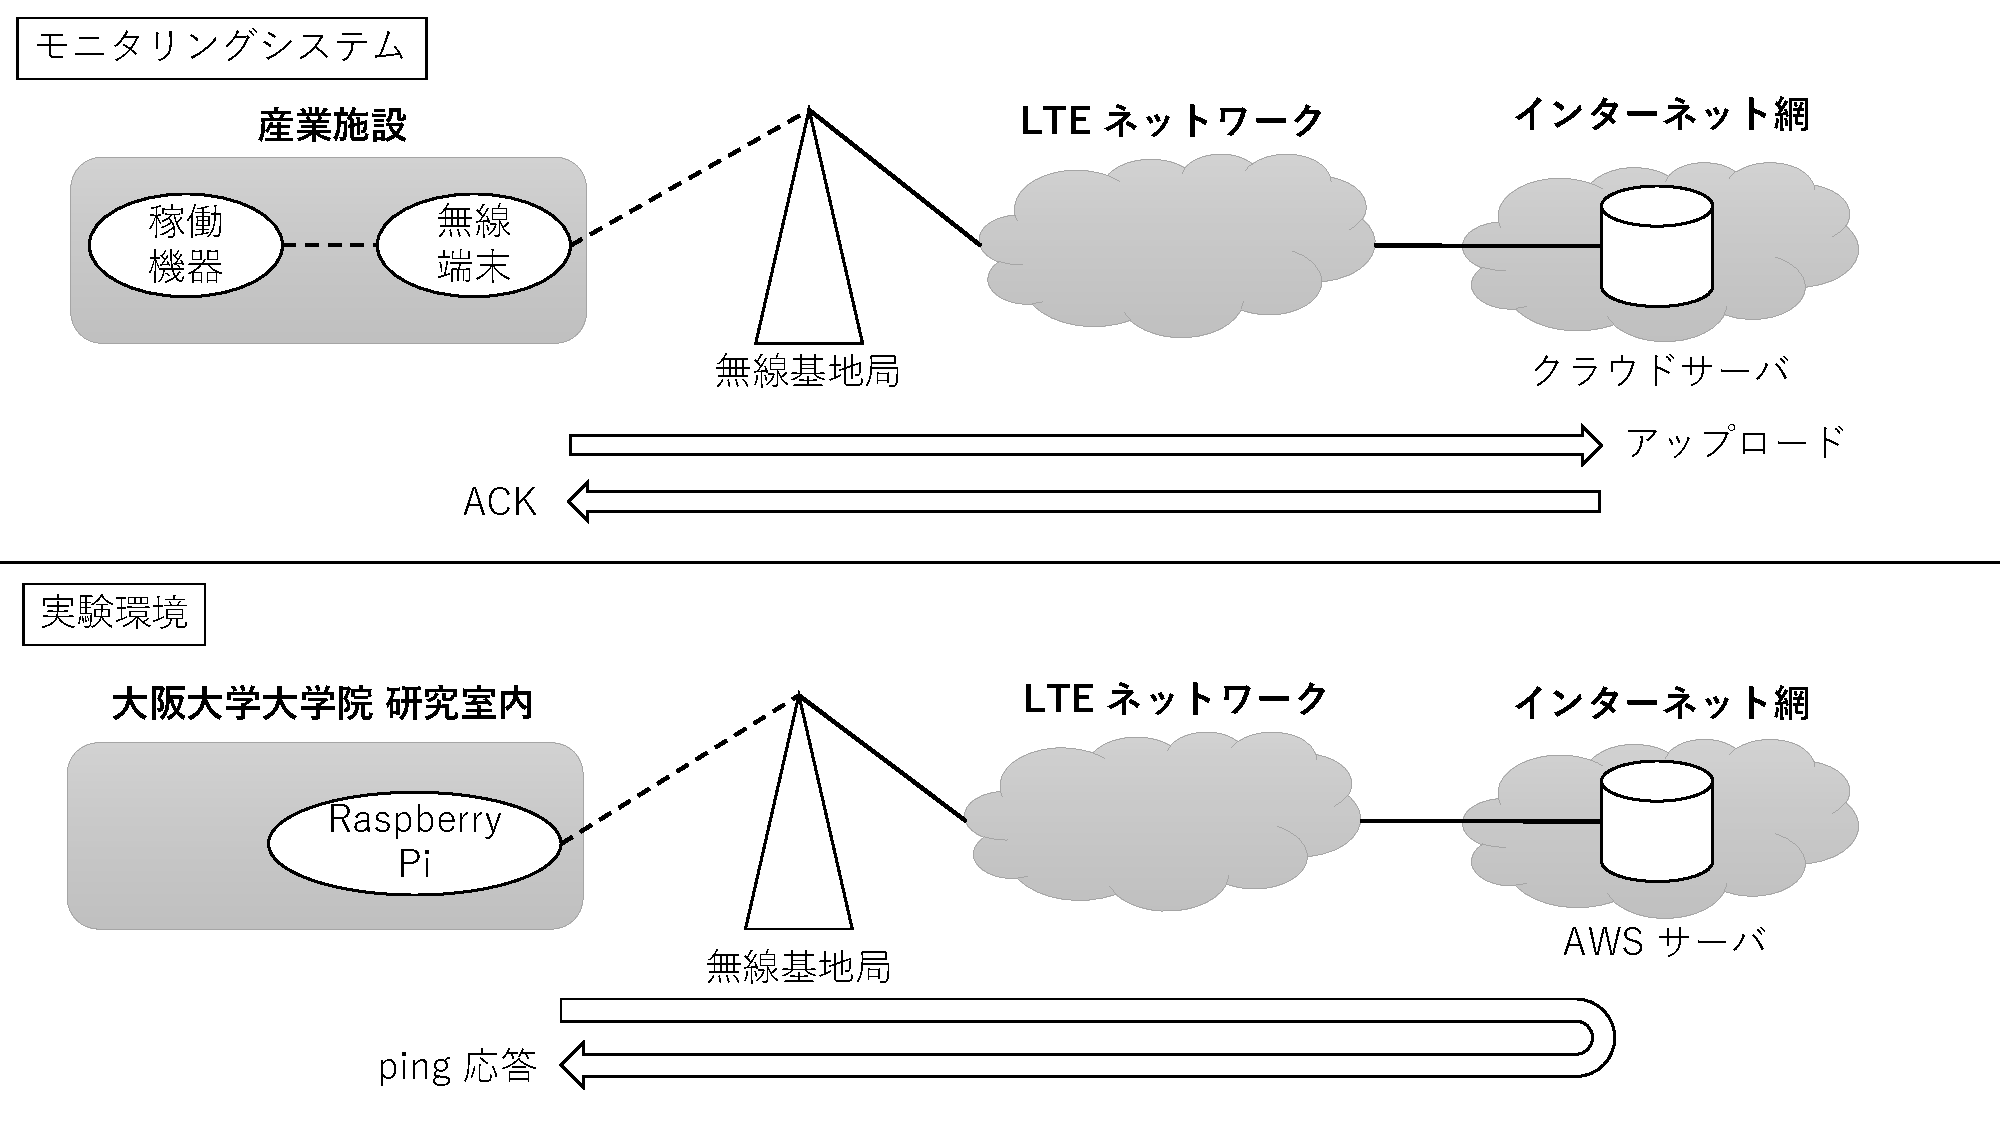
\includegraphics[width=7.5cm]{../figure/experiment.pdf}
\caption{モニタリングシステムと実験環境の対応図}
\label{exp}
\end{figure}

\section{時系列モデルによる回帰}
本報告では,時系列モデルとして式 (\ref{garch1}) と式 (\ref{garch2}) で表される ARMA-GARCH(Autoregressive Moving Average - Generalized Autoregressive Conditional Heteroscedasticity)モデルを用いる.
\begin{equation}
y_t = \sum_{i=1}^p a_i y_{t-i} + \sum_{i=1}^q b_i \varepsilon_{t-i} + c + \varepsilon_{t} \hspace{1.5cm}\varepsilon_t \sim N(0,h_t) \hspace{0.5cm} i.i.d
\label{garch1}
\end{equation}
\begin{equation}
\displaystyle h_{t} = \omega + \sum_{i=1}^{r}\alpha_i\varepsilon_{t-i}^2 + \sum_{i=1}^{s}\beta_ih_{t-i}
\label{garch2}
\end{equation}
本報告では,各一時間の計測実験において Raspberry Pi が AWS サーバから受け取る ping の応答遅延の実測値を計測時刻順に $y_1$,$y_2$,...,$y_N$ と表す.
式 (\ref{garch1}) において,$c$ は定数項,$\varepsilon_t$ はノイズ項であり平均 0 分散 $h_t$ の正規分布に従いそれらは互いに独立であるとし,時刻 $t$ における実測値 $y_t$ は,過去の $p$ 時点前までの実測値の線形和と $q$ 時点前までのノイズ項の加重和と自身のノイズ項によって表される.
また,式 (\ref{garch2}) において,$\omega$ は定数項であり,時刻 $t$ におけるノイズ項が従う正規分布の分散 $h_t$ は,過去の $r$ 時点前までのノイズ項の線形和と $s$ 時点前までのノイズ項が従う正規分布の分散の加重和によって表される.

各パラメータのパラメータ数 $(p,q,r,s)$ は次数と呼ばれ,精度の良い回帰を行うためには対象とする時系列データに応じてこの次数を適切に定める必要がある.
しかしながら,計測データのクラスタリングによる分類のためには異なる曜日や時間帯での計測によって得られた時系列データに対して次数を統一して回帰しなければならない.
そこで,本報告では,まず,各計測データに対し ARMA-GARCH モデルの次数を変えながら適用し,AIC(赤池情報量規準)によってその妥当性を評価することで,各時系列データにとって適切な次数を求める.
ここで,AIC は式(\ref{aic})で定められる指標である.
高すぎる次元での回帰による過適合の問題を考慮し,時系列モデルによる回帰のよさを評価する第 1 項とパラメータの少なさを評価する第 2 項を組み合わせている.
AICが小さいほどよいモデルとされている.
\begin{equation}
AIC = -2 *(対数尤度)+2 *(パラメータ数)
\label{aic}
\end{equation}
次に,各時系列データ間で AIC による最適次数を比較し,その最大のものを用いることとする.
次数の探索範囲は $0 \le p \le 2$,$0 \le q \le 2$,$r = 1$,$0 \le s \le 1$ とすると,統一する次数は $(p,q,r,s) = (2,2,1,1)$ となった.

また,応答遅延の変動に注目し,応答遅延の実測値の差分系列 $\{\Delta y_t | y_t - y_{t-1}\}$ に対しても同様にモデルの適用を行った.
統一する次数は $(p,q,r,s) = (2,2,1,1)$ となった.


\section{AWS サーバと SINET のウェブサーバを対象とした計測データのクラスタリング結果の比較}
 ARMA-GARCH モデルを実測値データもしくは変動値データに対して適用した結果定まるパラメータ $W$ をもとにクラスタリングを行い,時間帯や場所ごとの ping 応答遅延特性を分析する.
AWS サーバを対象とした計測データにおける $W$ は,実測値データと差分系列データともに
$$W = [c, a_1, a_2, b_1, b_2, \omega, \alpha_1, \beta_1] $$
で与えられ,SINET のウェブサーバを対象とした計測データにおける $W$ は,実測値データと差分系列データともに
$$W = [c, a_1, a_2, b_1, b_2, \omega, \alpha_1, \alpha_2, \beta_1, \beta_2] $$
で与えられる.
SINET のものに関しては卒論時と合わせています.
SINET を対象とした実測値データにおいて ARMA-GARCH の適用ができないものに関しては省いて行っております.
また,AWS サーバを対象とした計測データは 2/29(土)から3/27(金)までに計測したものを用い,SINET のウェブサーバを対象とした計測データは 12/29(火)から 1/30(木)までに計測したものを用いる.

ここでは,距離関数をユークリッド距離とし,クラスタ融合手法としてウォード法を用いる.
クラスタ数は 6,7,9,12,15 とした.

さらに標準化を行ったパラメータの主成分でのクラスタリングも行う.
これは,パラメータ間で大きさや分散が異なること,次元数が多いことによりクラスタリングの精度が低下する可能性を考え,その対処として行った.
AWS サーバと SINET のウェブサーバを対象とした計測データにおける実測値データと変動値データの主成分分析におけるそれぞれの累積寄与率は表 \ref{comp-summary-1} から表 \ref{comp-summary-2} となっており,累積寄与率が 70\% を超えた主成分までを用いてクラスタリングを行う.
従って,AWS サーバを対象とした実測値と変動値,SINET のウェブサーバを対象とした実測値に対してはその第三主成分まで,SINET のウェブサーバを対象とした変動値に対してはその第四主成分までを用いる.
この時の各主成分の負荷量は表 \ref{comp-loading-1} から表 \ref{comp-loading-2} となっていた.

\begin{table}[tb]
\centering
\caption{AWS サーバを対象とした実測値の主成分分析における累積寄与率}
\label{comp-summary-1}
\begin{tabular}{|l|l|l|l|}
\hline
第一主成分&第二主成分&第三主成分&第四主成分\\
\hline
0.449& 0.681& 0.863& 0.968\\
\hline
\end{tabular}
\caption{AWS サーバを対象とした変動値の主成分分析における累積寄与率}
\begin{tabular}{|l|l|l|l|}
\hline
第一主成分&第二主成分&第三主成分&第四主成分\\
\hline
0.367& 0.653& 0.794& 0.905\\
\hline
\end{tabular}
\caption{SINET のウェブサーバを対象とした実測値の主成分分析における累積寄与率}
\begin{tabular}{|l|l|l|l|}
\hline
第一主成分&第二主成分&第三主成分&第四主成分\\
\hline
0.324& 0.556& 0.718& 0.834\\
\hline
\end{tabular}
\caption{SINET のウェブサーバを対象とした変動値の主成分分析における累積寄与率}
\label{comp-summary-2}
\begin{tabular}{|l|l|l|l|l|}
\hline
第一主成分&第二主成分&第三主成分&第四主成分&第五主成分\\
\hline
0.308& 0.497& 0.648& 0.768&0.879\\
\hline
\end{tabular}
\end{table}

\begin{table}[tb]
\centering
\begin{minipage}[t]{.45\textwidth}
\caption{AWS サーバを対象とした実測値の負荷量}
\label{comp-loading-1}
\begin{tabular}{|l|l|l|l|}
\hline
&第一主成分&第二主成分&第三主成分\\
\hline
$c$&0.515&0.133& \\
$a_1$&-0.418&&-0.490\\
$a_2$&-0.404&-0.166&0.492\\
$b_1$&0.424&&0.475\\
$b_2$&0.391&0.157&-0.516\\
$\omega$&-0.119&0.569&0.101\\
$\alpha_1$&-0.142&0.432&\\
$\beta_1$&0.175&-0.643&-0.111\\
\hline
\end{tabular}
\end{minipage}
\hfill
\begin{minipage}[t]{.45\textwidth}
\caption{AWS サーバを対象とした変動値の負荷量}
\begin{tabular}{|l|l|l|l|}
\hline
&第一主成分&第二主成分&第三主成分\\
\hline
$c$&&&0.721\\
$a_1$&0.571&&\\
$a_2$&&-0.190&-0.067\\
$b_1$&-0.571&&\\
$b_2$&0.574&&\\
$\omega$&&0.553&-0.127\\
$\alpha_1$&&0.499&\\
$\beta_1$&&-0.629&\\
\hline
\end{tabular}
\end{minipage}

\begin{minipage}[t]{.45\textwidth}
\caption{SINET のウェブサーバを対象とした実測値の負荷量}
\begin{tabular}{|l|l|l|l|}
\hline
&第一主成分&第二主成分&第三主成分\\
\hline
$c$&0.546&& \\
$a_1$&-0.374&-0.423&-0.150\\
$a_2$&-0.441&&0.283\\
$b_1$&0.352&0.448&0.154\\
$b_2$&0.443&-0.288&\\
$\omega$&&0.349&-0.526 \\
$\alpha_1$&&0.328&-0.294\\
$\alpha_2$&&0.178&-0.166\\
$\beta_1$&0.163&-0.430&-0.209 \\
$\beta_2$&&&0.708\\
\hline
\end{tabular}
\end{minipage}
\hfill
\begin{minipage}[t]{.45\textwidth}
\caption{SINET のウェブサーバを対象とした変動値の負荷量}
\label{comp-loading-2}
\begin{tabular}{|l|l|l|l|l|}
\hline
&第一主成分&第二主成分&第三主成分&第四主成分\\
\hline
$c$&&0.346&0.142&0.465\\
$a_1$&-0.552&&&-0.123\\
$a_2$&&-0.371&-0.144&-0.482\\
$b_1$&0.544&-0.128&-0.103&0.112 \\
$b_2$&-0.546&0.140&&-0.111\\
$\omega$&-0.204&-0.490&-0.328&0.250 \\
$\alpha_1$&-0.199&-0.290&&0.598\\
$\alpha_2$&&-0.226&-0.154&-0.248\\
$\beta_1$&&0.560&-0.456&-0.132 \\
$\beta_2$&0.122&-0.114&0.771&-0.116\\
\hline
\end{tabular}
\end{minipage}
\end{table}

以下その結果を図 \ref{cluster1} から図 \ref{cluster2} に示す.
このそれぞれは,該当するクラスタリングによって分類された計測データを,計測した時間帯もしくは曜日ごとに色分けした積み上げ棒グラフ,および計測した曜日と時間帯が同じ計測データを属するクラスタごとに色分けした積み上げ棒グラフである.
前者の縦軸は各クラスタ内の個数に対する割合であり,上部に各クラスタに属する計測データの個数を示しており,後者の縦軸は曜日と時間帯が同じデータが属するクラスタの割合であり,上部に各曜日と時間帯のデータ数を示している.

\begin{figure}[tb]
\begin{center}
\subfigure[クラスタ数 6 : 時間帯]{
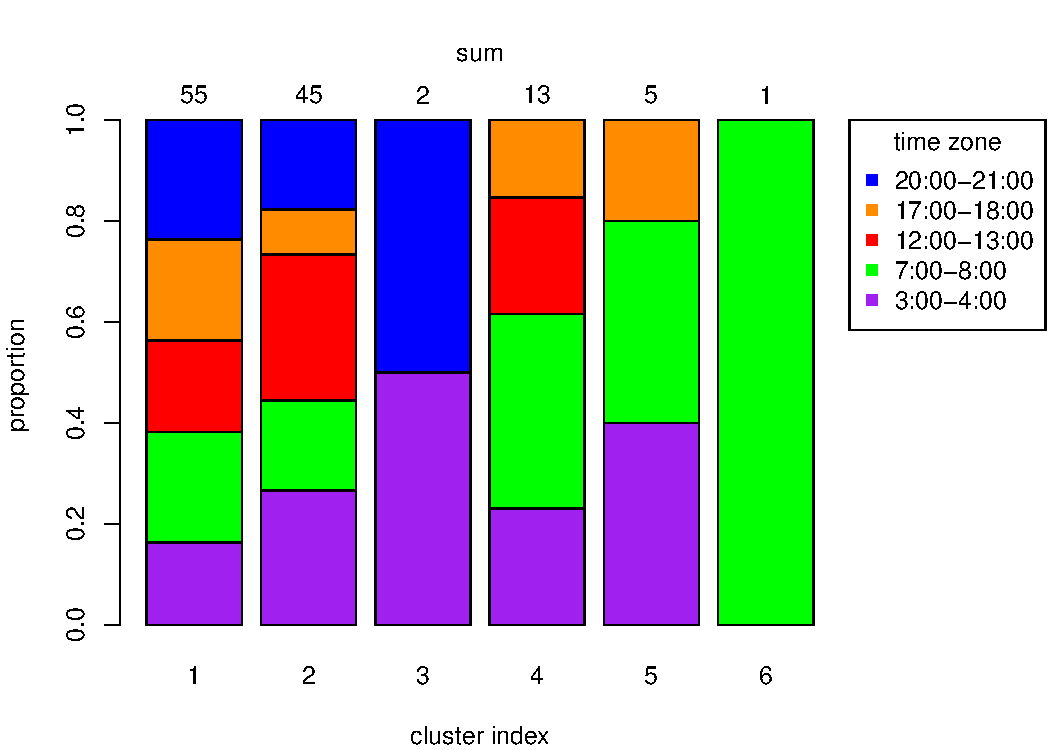
\includegraphics[height=3.5cm,width=5cm]{norm-eucl-ward-6-timezone.pdf}
}~
\subfigure[クラスタ数 6 : 曜日]{
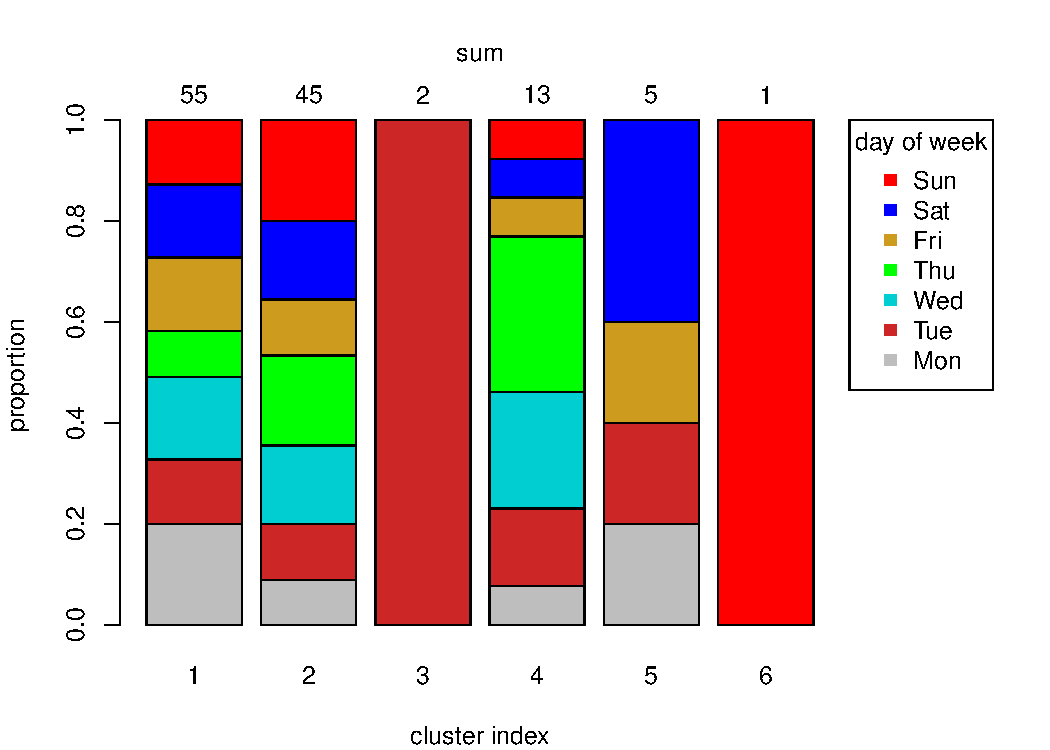
\includegraphics[height=3.5cm,width=5cm]{norm-eucl-ward-6-day.pdf}
}~
\subfigure[クラスタ数 6 : 時間帯と曜日]{
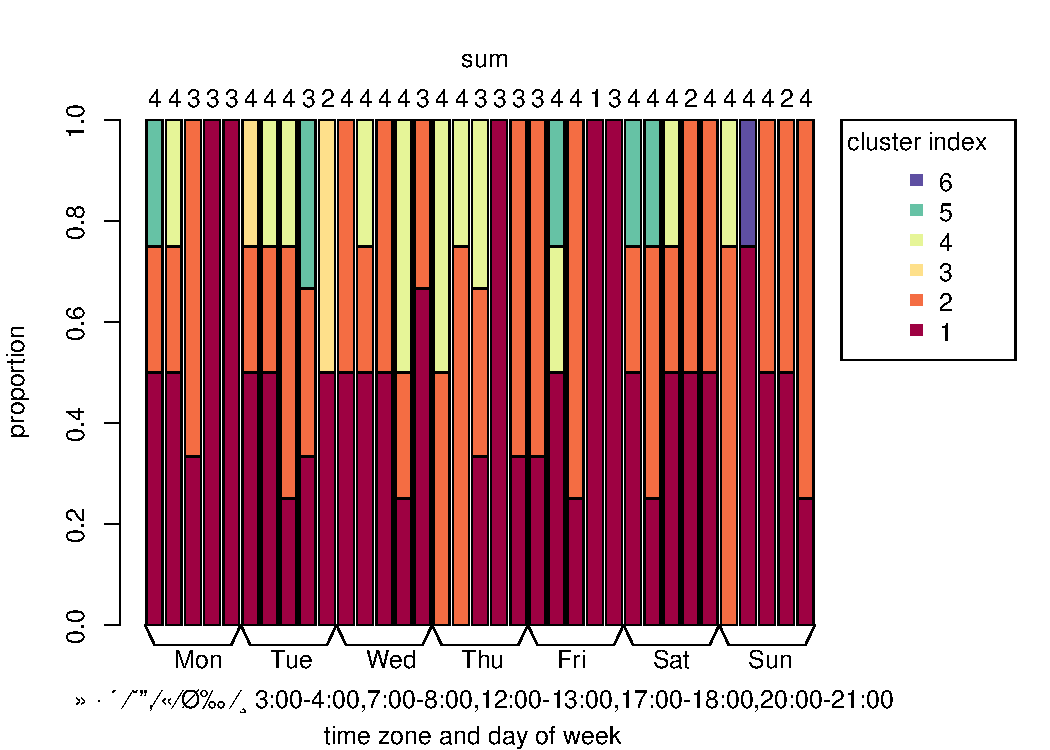
\includegraphics[height=3.5cm,width=5cm]{norm-eucl-ward-6-timezone-day.pdf}
}\\
\subfigure[クラスタ数 7 : 時間帯]{
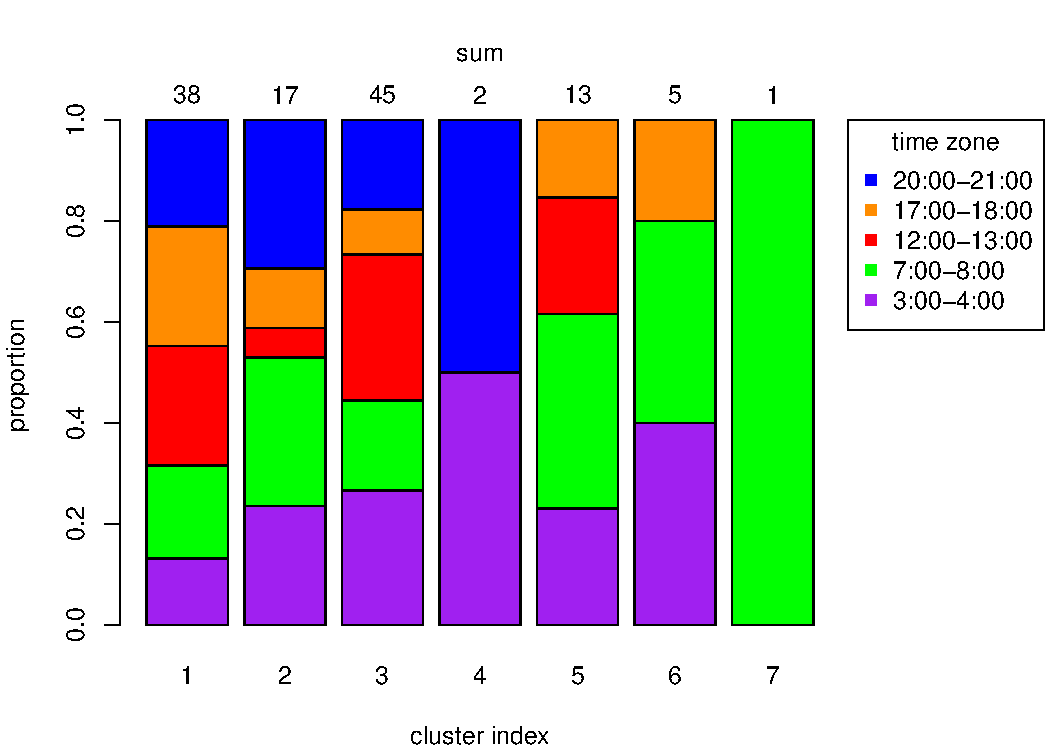
\includegraphics[height=3.5cm,width=5cm]{norm-eucl-ward-7-timezone.pdf}
}~
\subfigure[クラスタ数 7 : 曜日]{
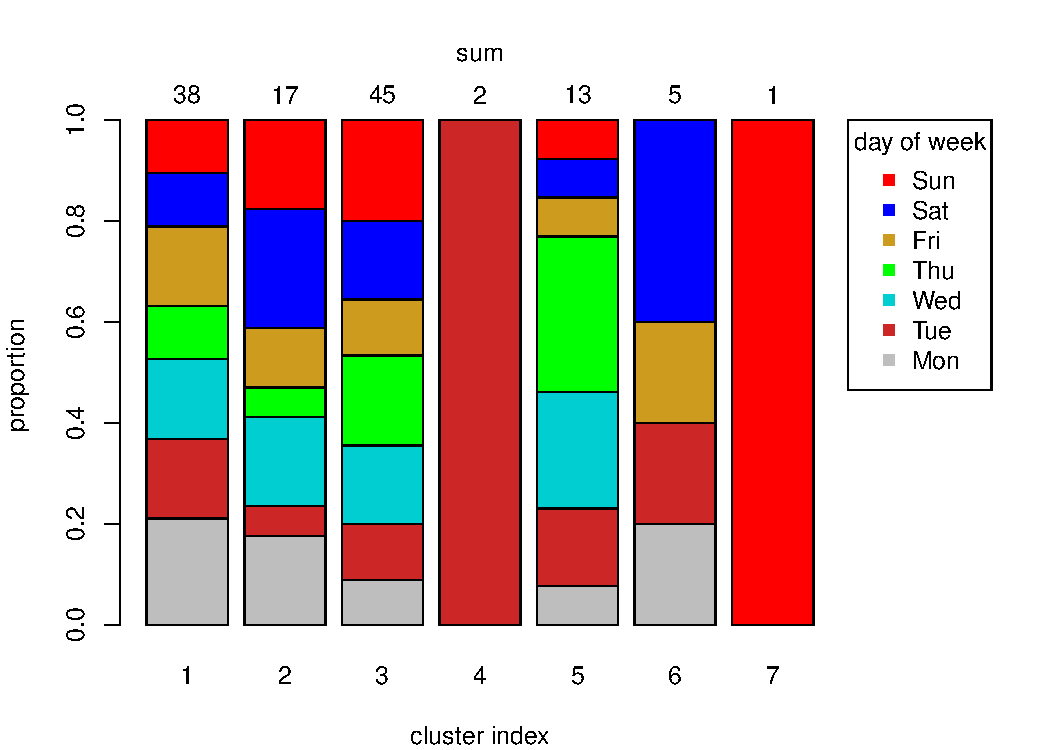
\includegraphics[height=3.5cm,width=5cm]{norm-eucl-ward-7-day.pdf}
}~
\subfigure[クラスタ数 7 : 時間帯と曜日]{
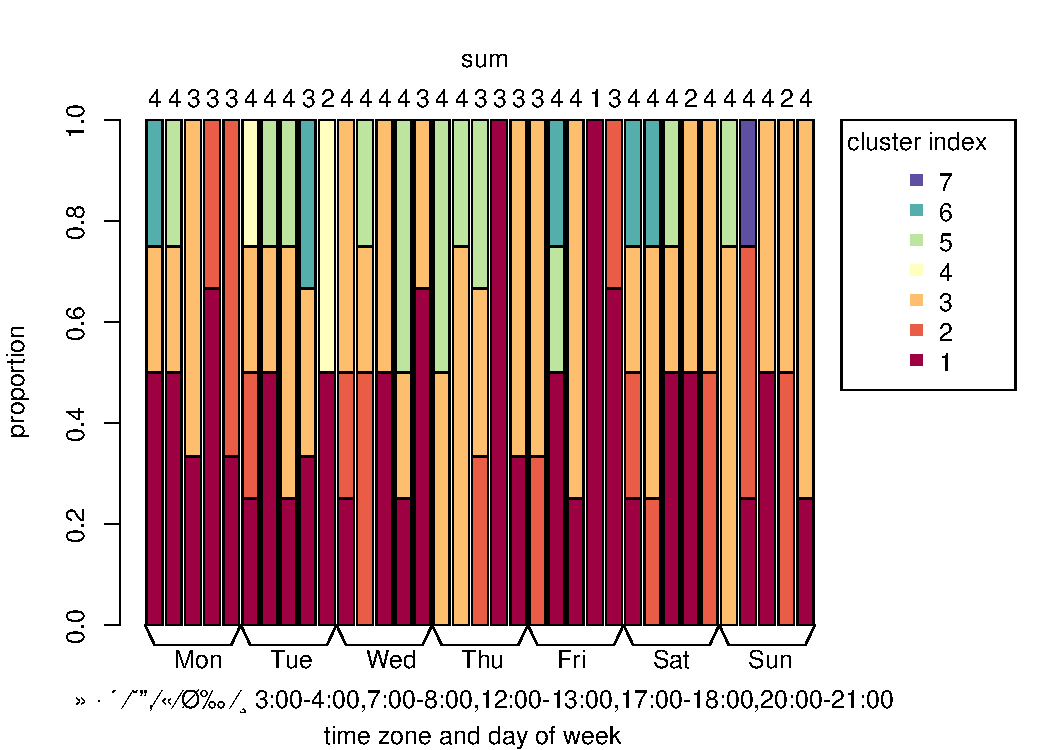
\includegraphics[height=3.5cm,width=5cm]{norm-eucl-ward-7-timezone-day.pdf}
}\\
\subfigure[クラスタ数 9 : 時間帯]{
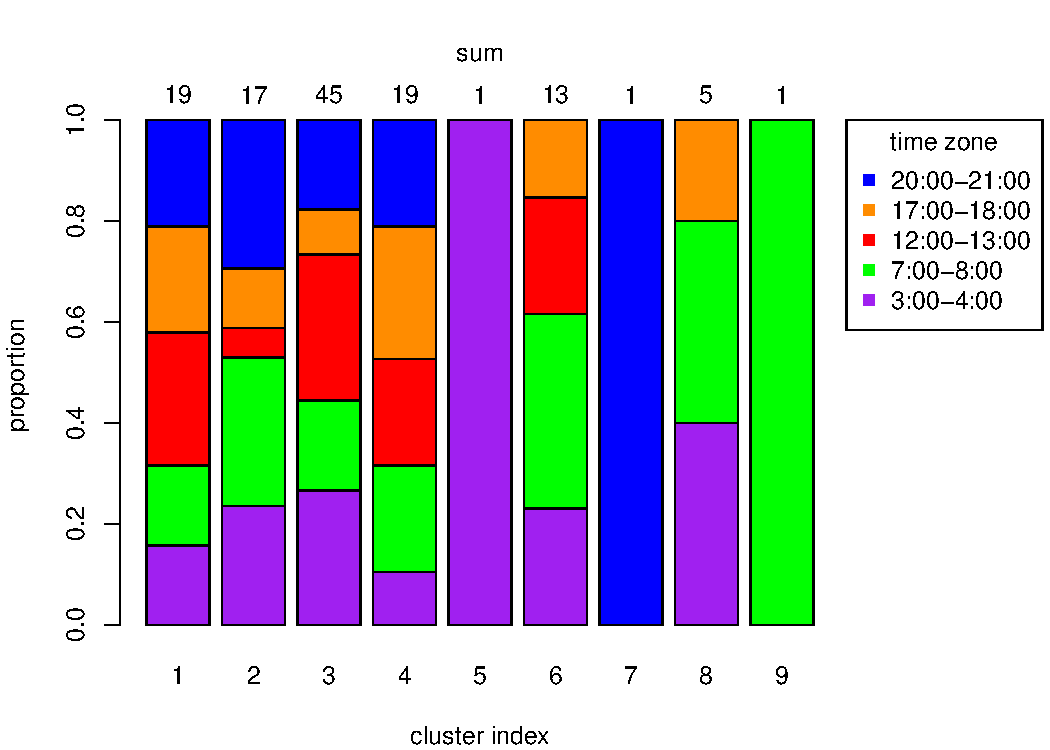
\includegraphics[height=3.5cm,width=5cm]{norm-eucl-ward-9-timezone.pdf}
}~
\subfigure[クラスタ数 9 : 曜日]{
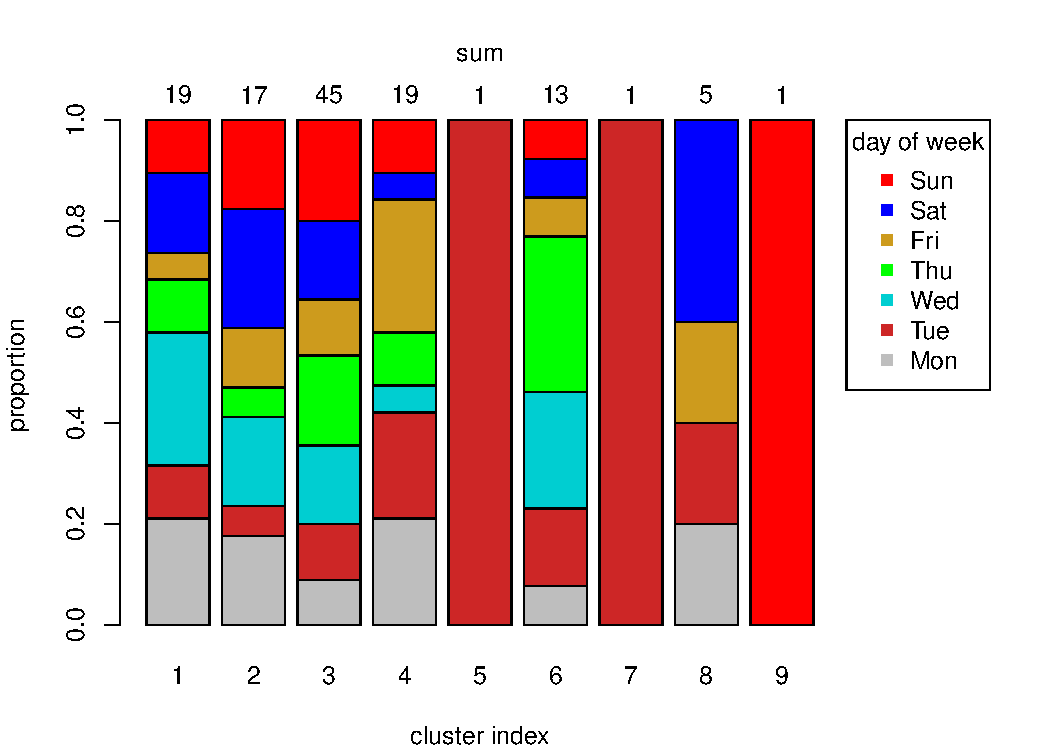
\includegraphics[height=3.5cm,width=5cm]{norm-eucl-ward-9-day.pdf}
}~
\subfigure[クラスタ数 9 : 時間帯と曜日]{
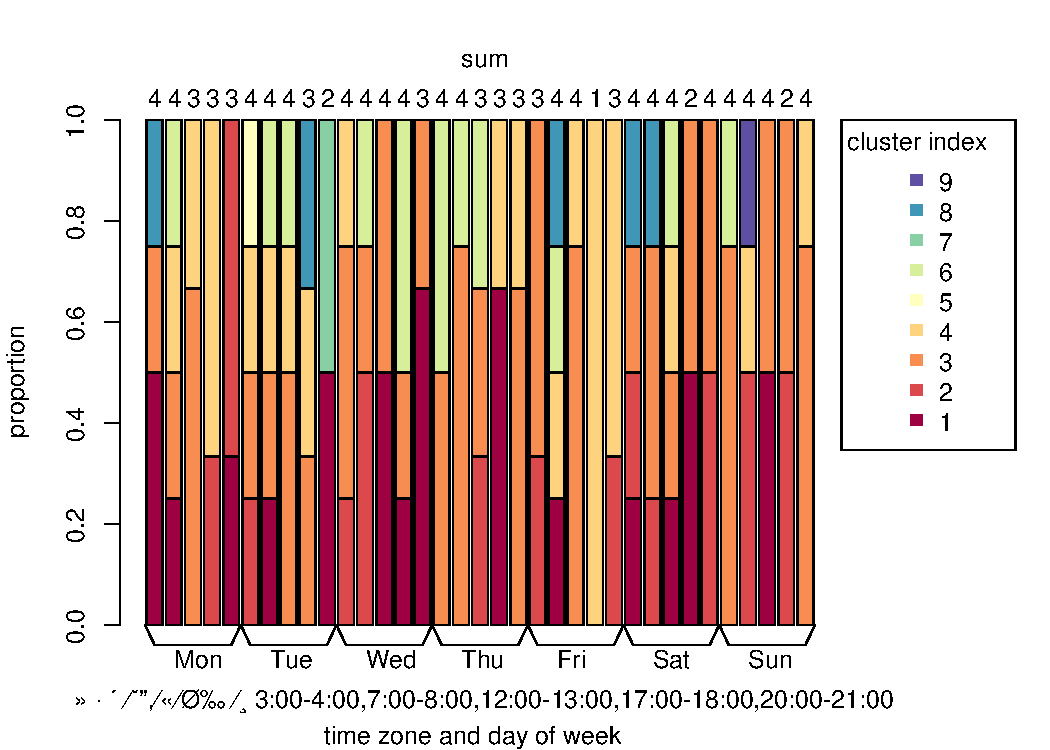
\includegraphics[height=3.5cm,width=5cm]{norm-eucl-ward-9-timezone-day.pdf}
}\\
\subfigure[クラスタ数 12 : 時間帯]{
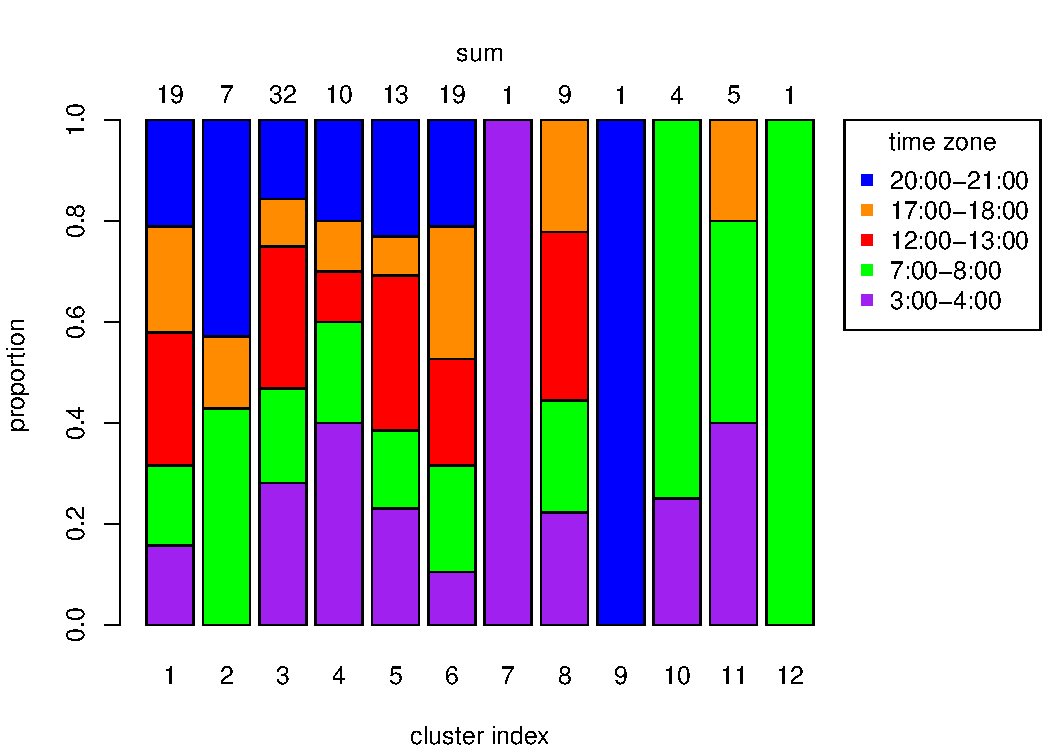
\includegraphics[height=3.5cm,width=5cm]{norm-eucl-ward-12-timezone.pdf}
}~
\subfigure[クラスタ数 12 : 曜日]{
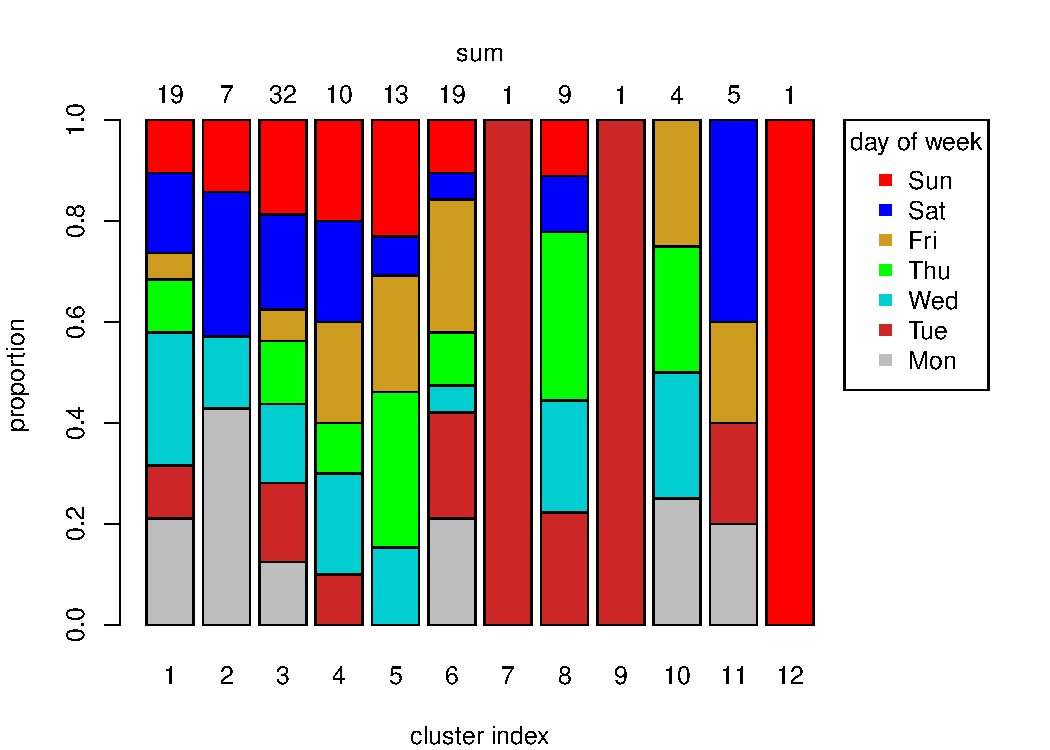
\includegraphics[height=3.5cm,width=5cm]{norm-eucl-ward-12-day.pdf}
}~
\subfigure[クラスタ数 12 : 時間帯と曜日]{
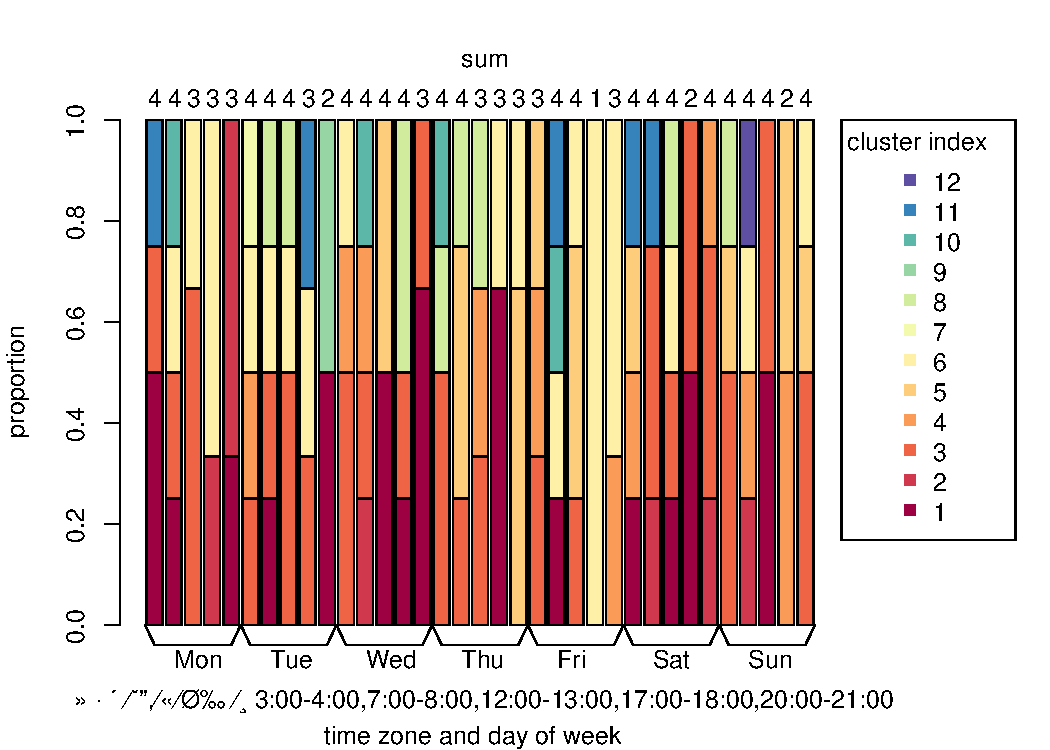
\includegraphics[height=3.5cm,width=5cm]{norm-eucl-ward-12-timezone-day.pdf}
}\\
\subfigure[クラスタ数 15 : 時間帯]{
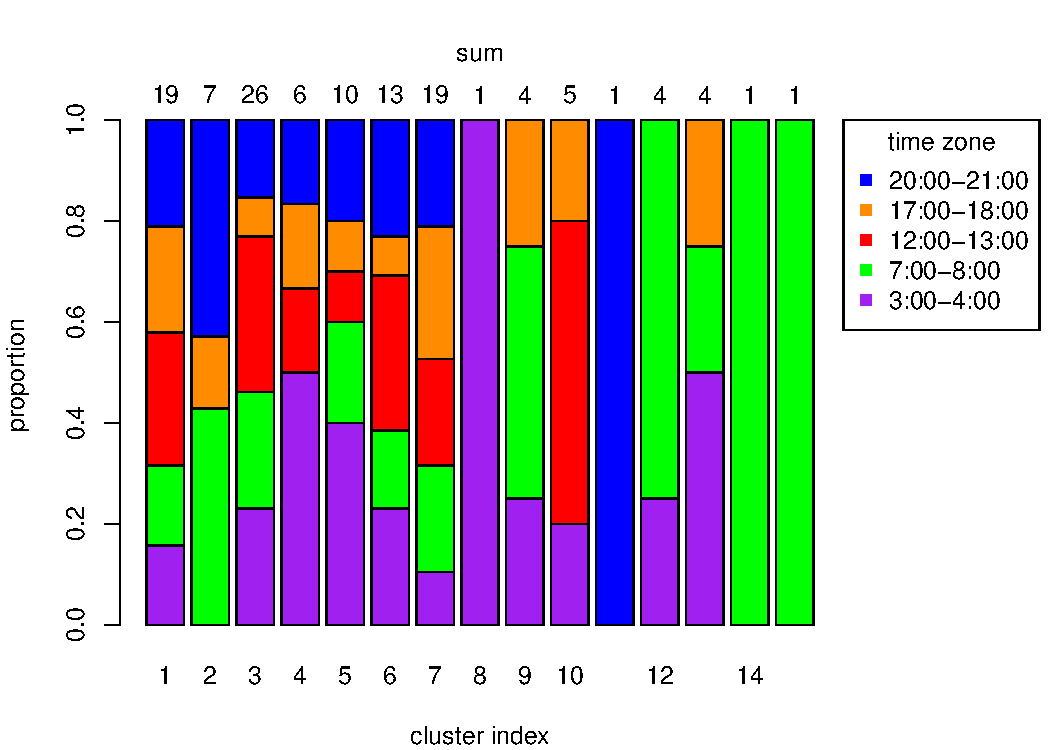
\includegraphics[height=3.5cm,width=5cm]{norm-eucl-ward-15-timezone.pdf}
}~
\subfigure[クラスタ数 15 : 曜日]{
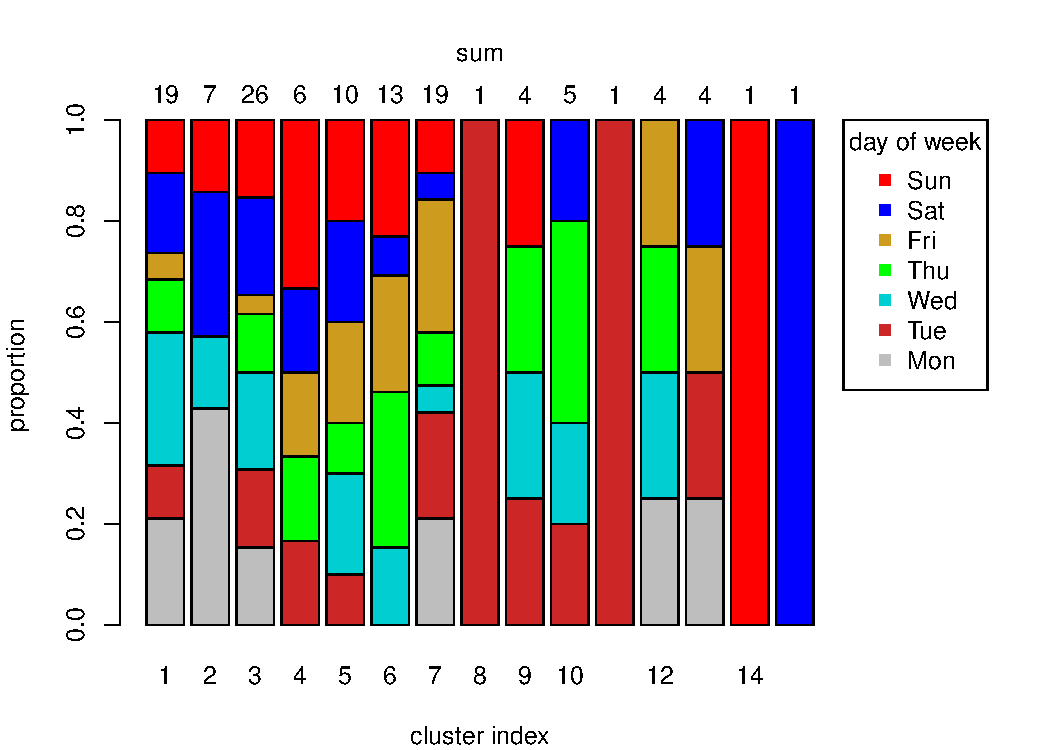
\includegraphics[height=3.5cm,width=5cm]{norm-eucl-ward-15-day.pdf}
}~
\subfigure[クラスタ数 15 : 時間帯と曜日]{
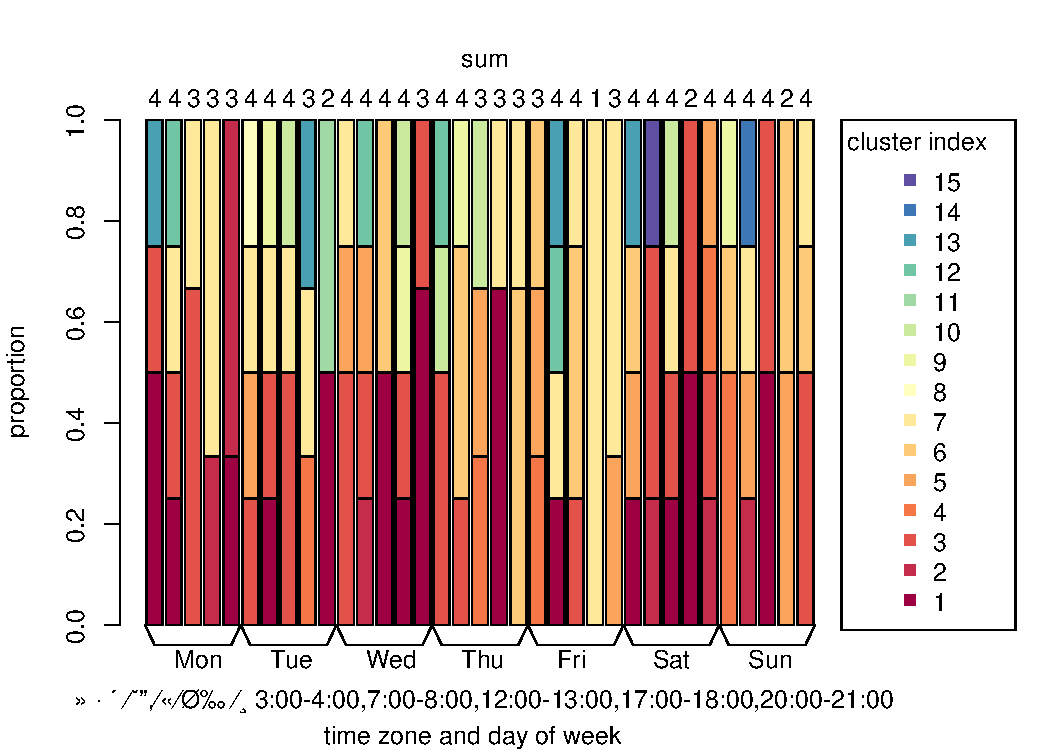
\includegraphics[height=3.5cm,width=5cm]{norm-eucl-ward-15-timezone-day.pdf}
}\\
\caption{AWS サーバを対象とした計測の実測値によるクラスタリング}
\label{cluster1}
\end{center}
\end{figure}

\begin{figure}[tb]
\begin{center}
\subfigure[クラスタ数 6 : 時間帯]{
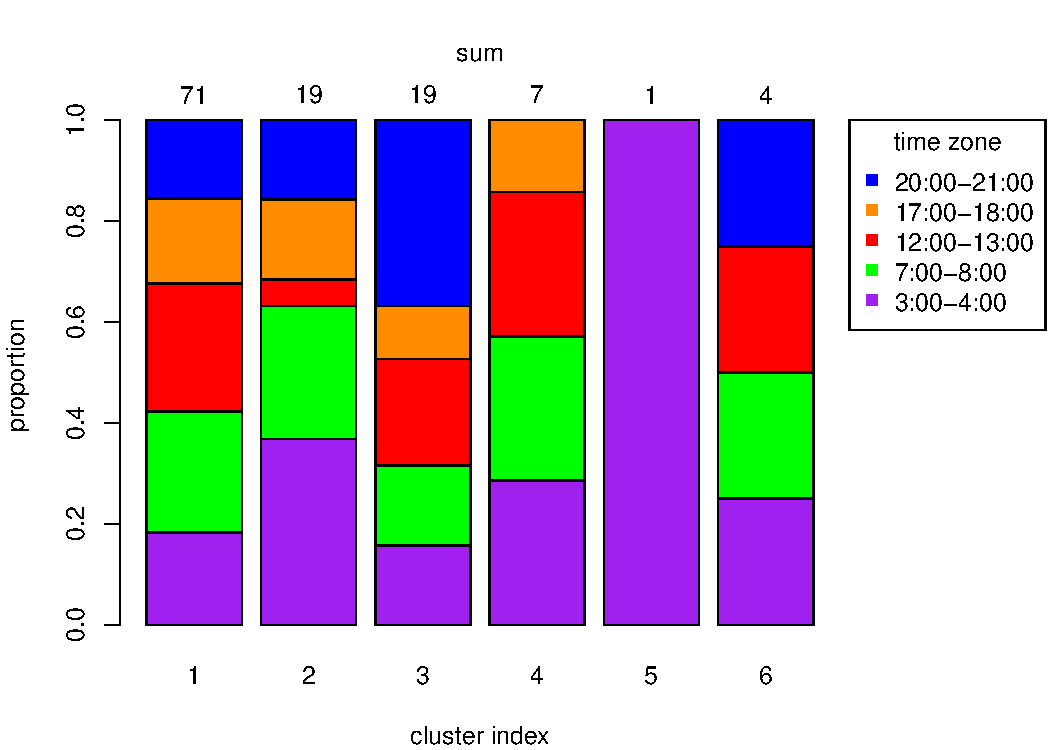
\includegraphics[height=3.5cm,width=5cm]{diff-eucl-ward-6-timezone.pdf}
}~
\subfigure[クラスタ数 6 : 曜日]{
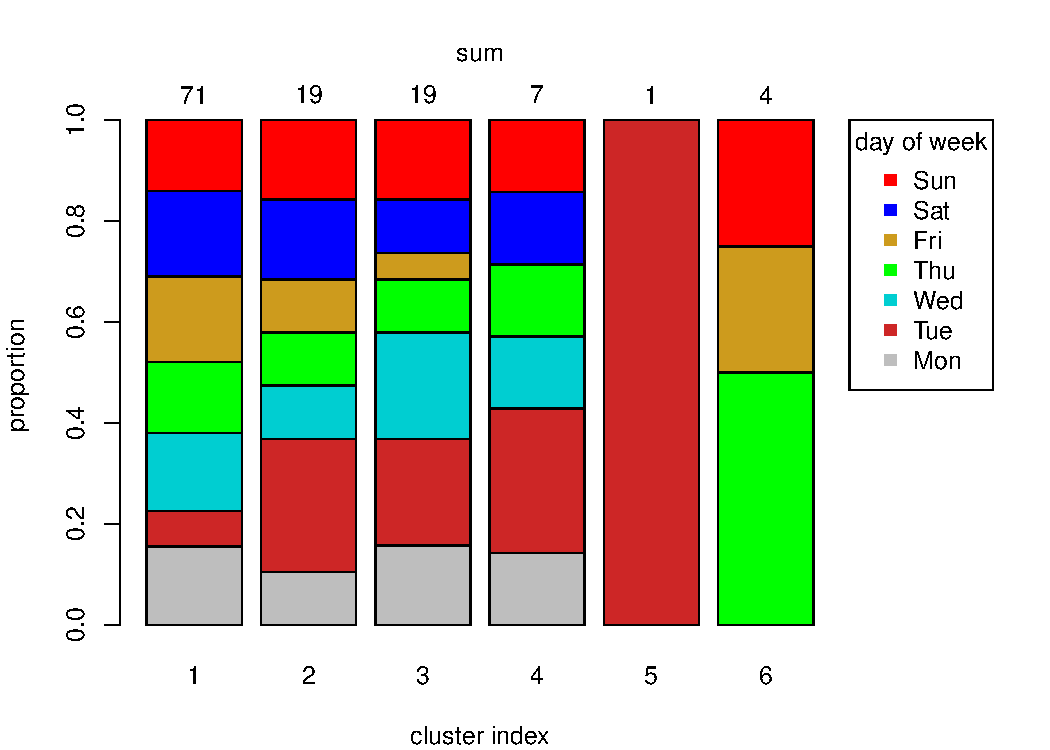
\includegraphics[height=3.5cm,width=5cm]{diff-eucl-ward-6-day.pdf}
}~
\subfigure[クラスタ数 6 : 時間帯と曜日]{
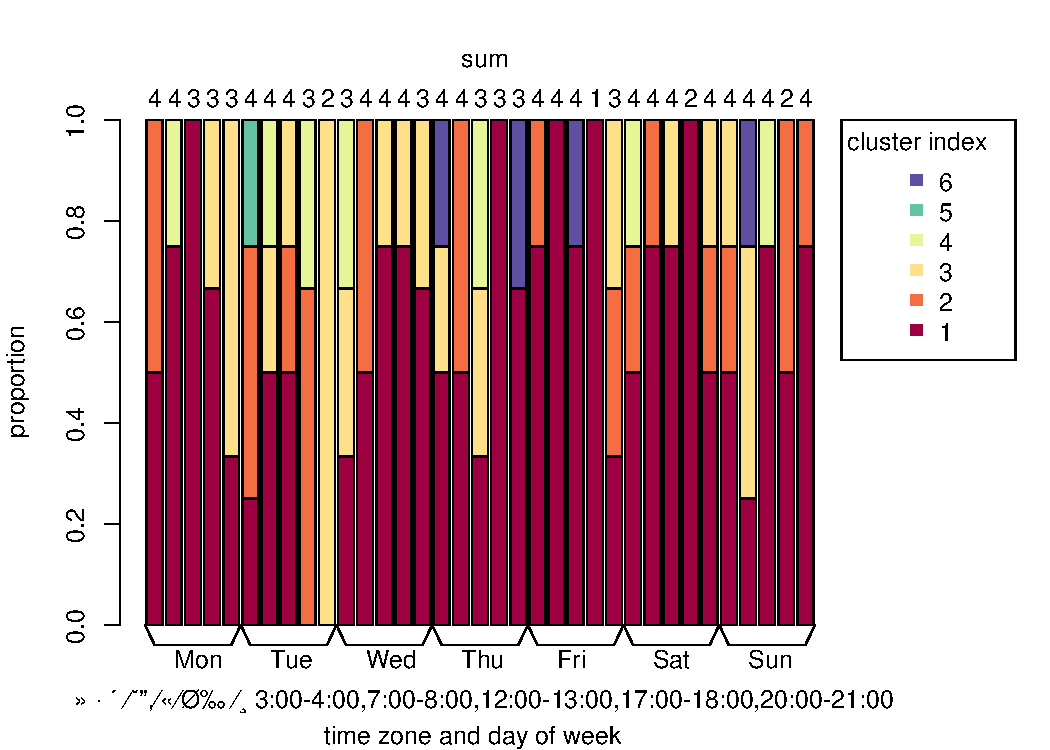
\includegraphics[height=3.5cm,width=5cm]{diff-eucl-ward-6-timezone-day.pdf}
}\\
\subfigure[クラスタ数 7 : 時間帯]{
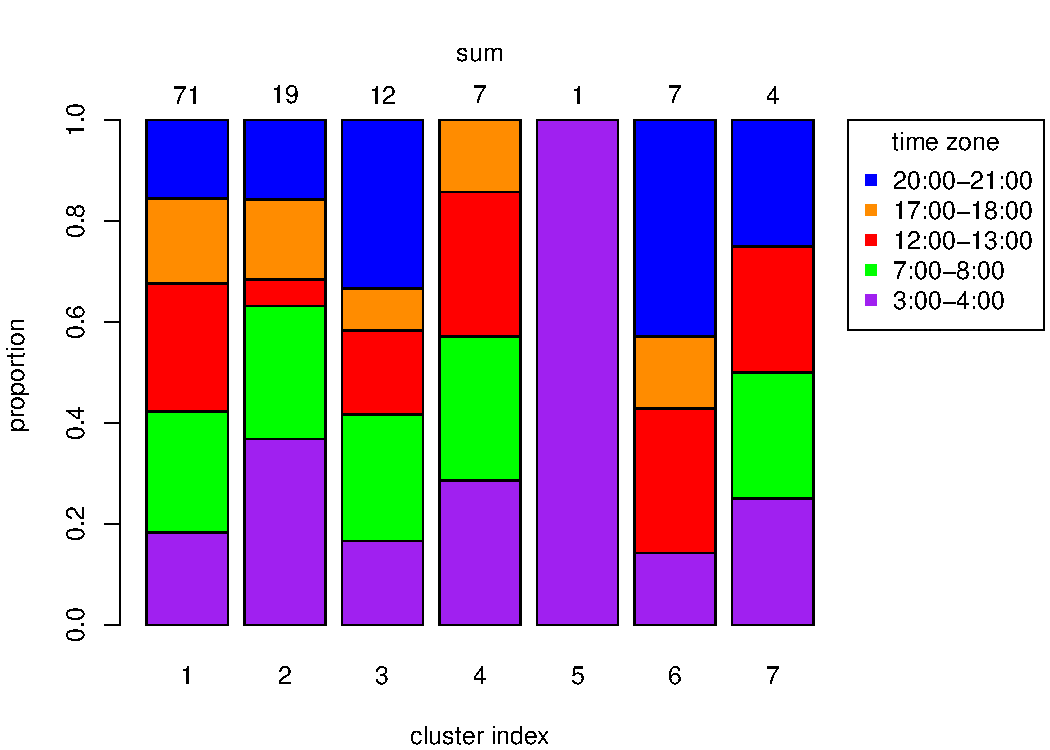
\includegraphics[height=3.5cm,width=5cm]{diff-eucl-ward-7-timezone.pdf}
}~
\subfigure[クラスタ数 7 : 曜日]{
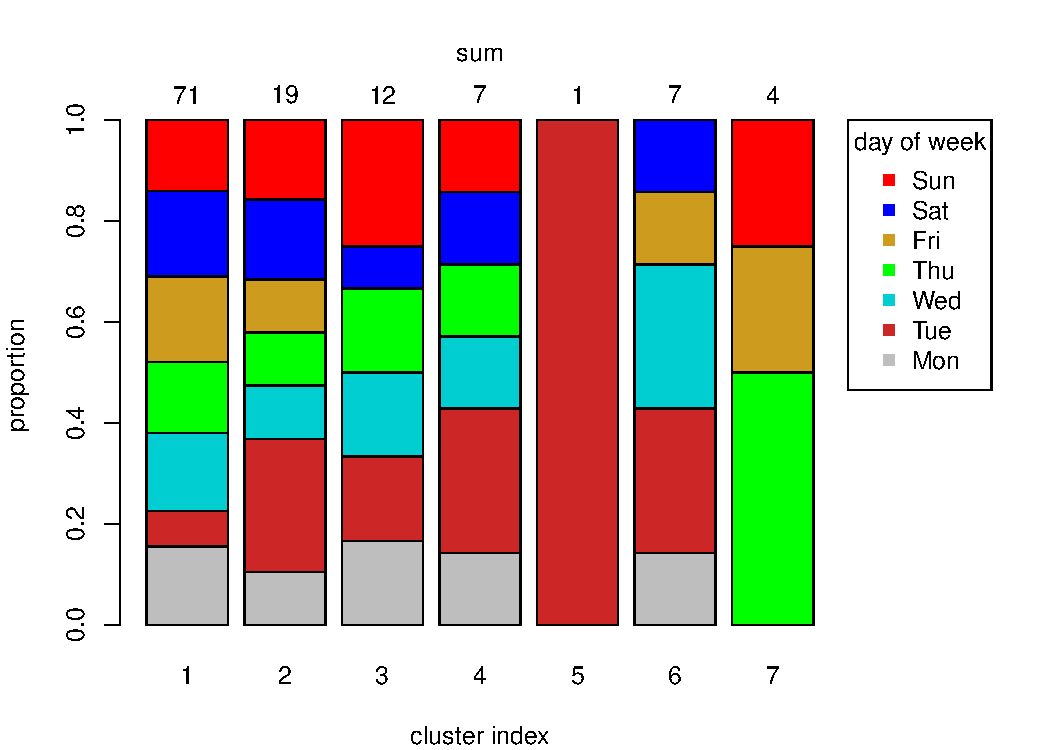
\includegraphics[height=3.5cm,width=5cm]{diff-eucl-ward-7-day.pdf}
}~
\subfigure[クラスタ数 7 : 時間帯と曜日]{
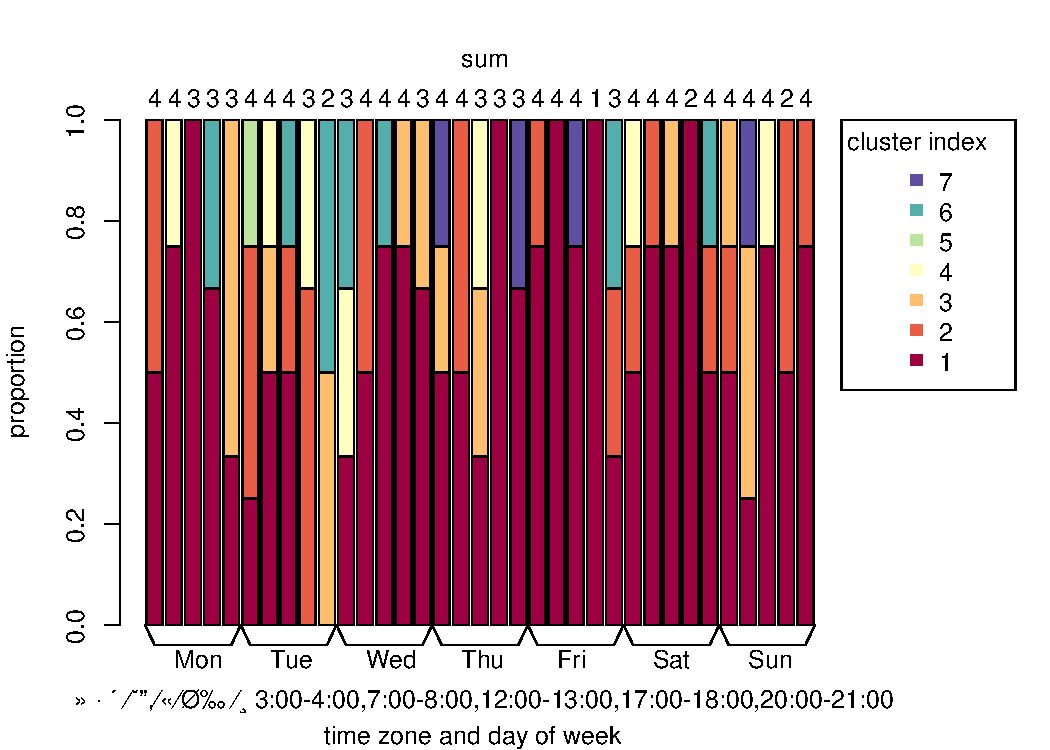
\includegraphics[height=3.5cm,width=5cm]{diff-eucl-ward-7-timezone-day.pdf}
}\\
\subfigure[クラスタ数 9 : 時間帯]{
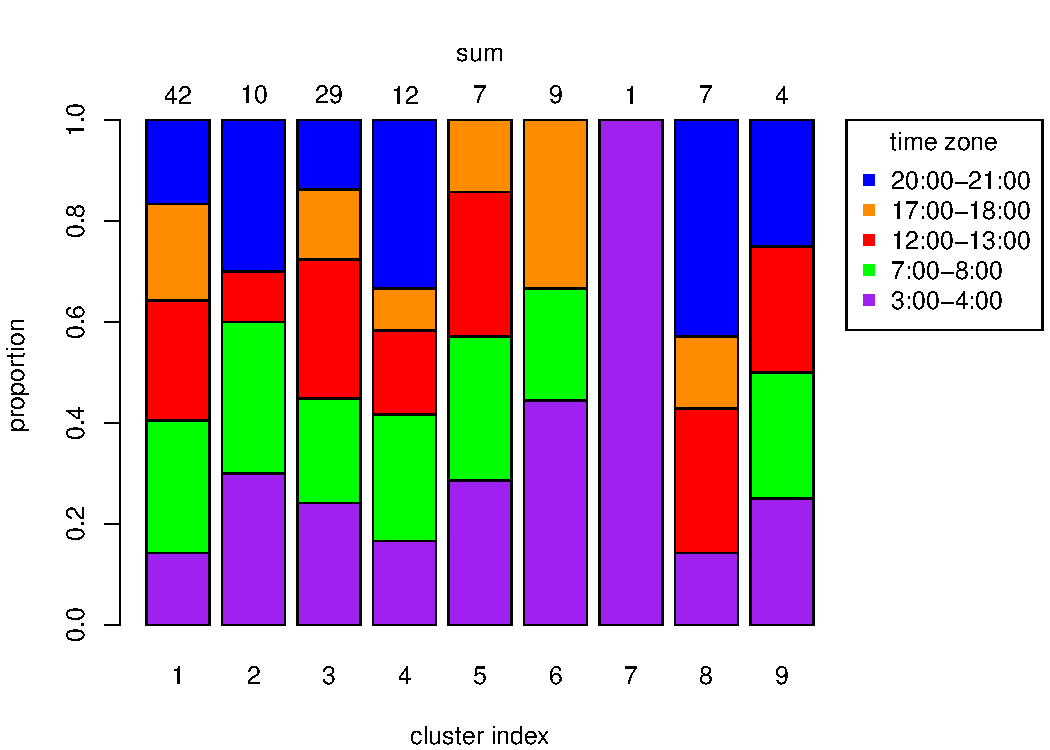
\includegraphics[height=3.5cm,width=5cm]{diff-eucl-ward-9-timezone.pdf}
}~
\subfigure[クラスタ数 9 : 曜日]{
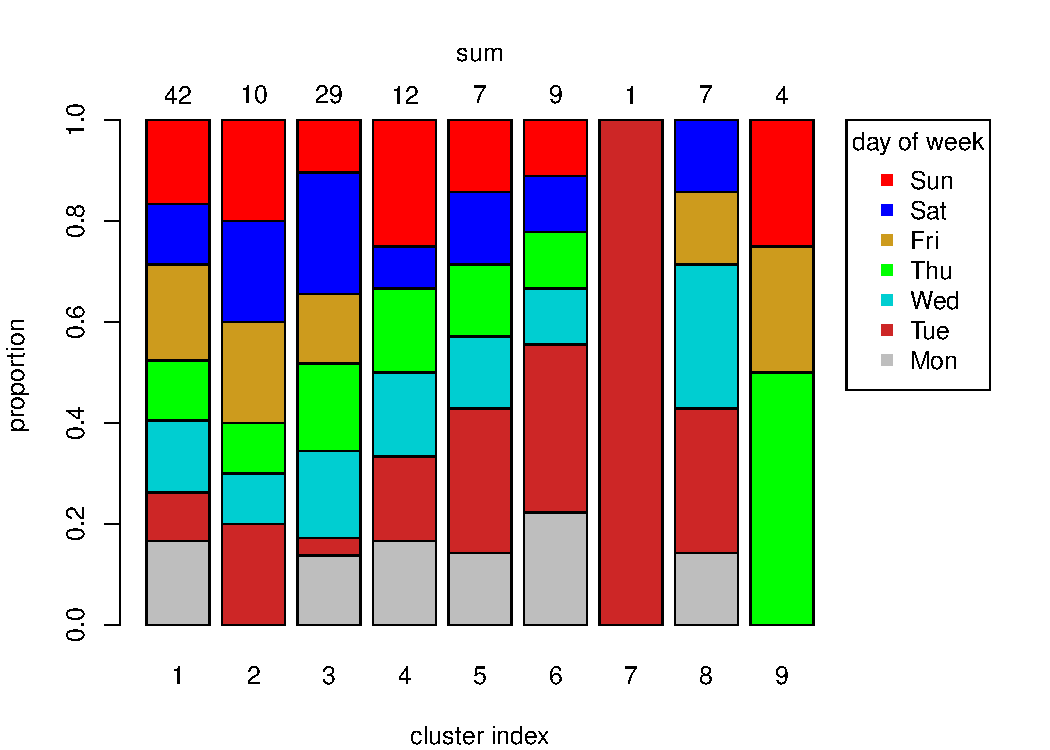
\includegraphics[height=3.5cm,width=5cm]{diff-eucl-ward-9-day.pdf}
}~
\subfigure[クラスタ数 9 : 時間帯と曜日]{
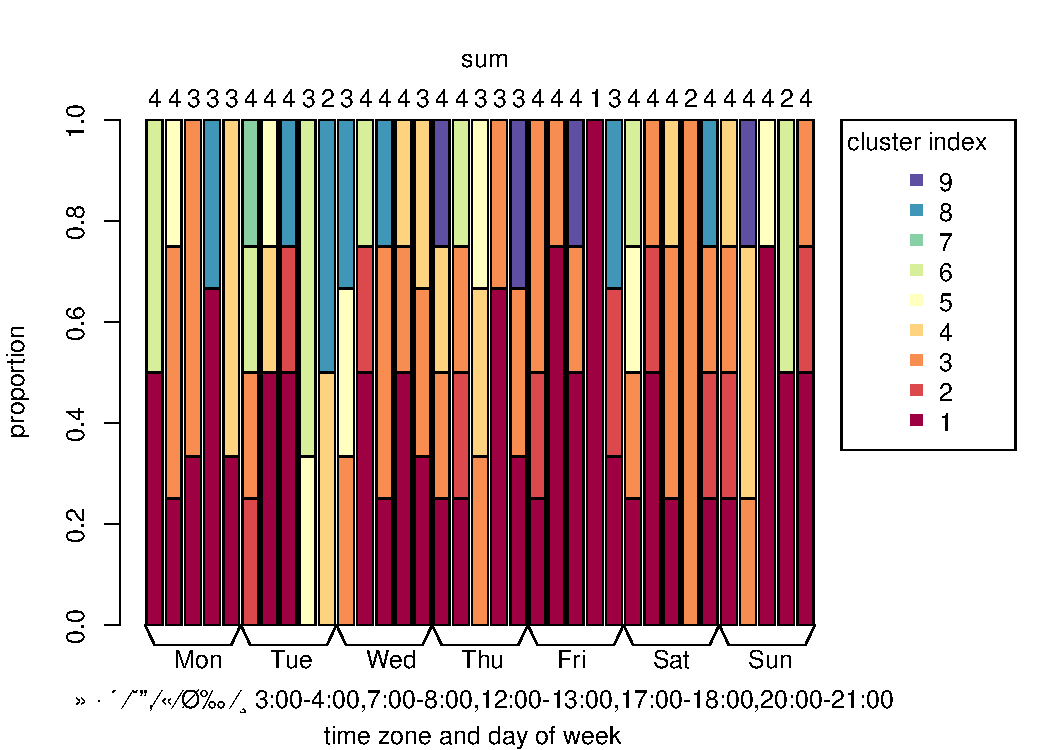
\includegraphics[height=3.5cm,width=5cm]{diff-eucl-ward-9-timezone-day.pdf}
}\\
\subfigure[クラスタ数 12 : 時間帯]{
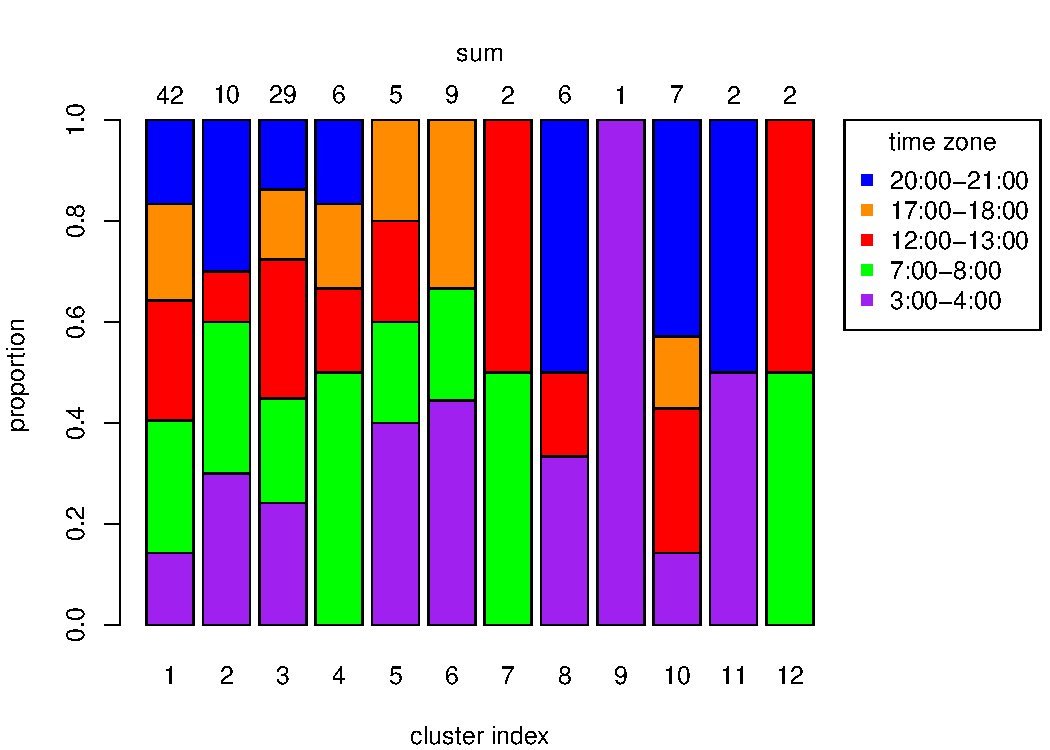
\includegraphics[height=3.5cm,width=5cm]{diff-eucl-ward-12-timezone.pdf}
}~
\subfigure[クラスタ数 12 : 曜日]{
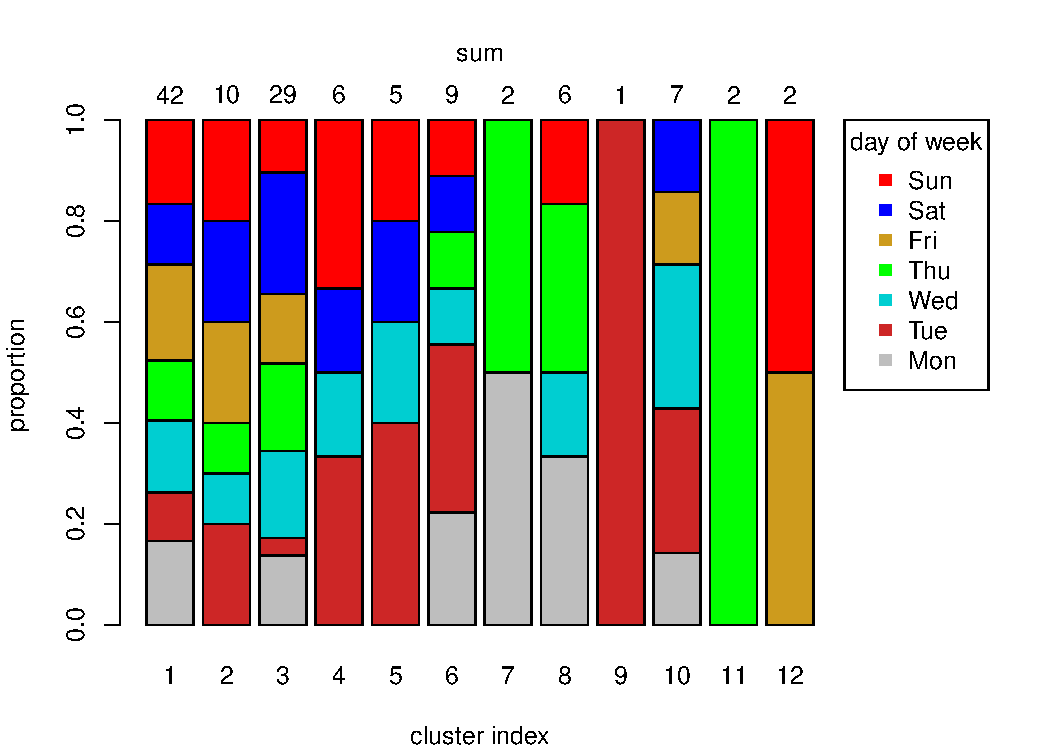
\includegraphics[height=3.5cm,width=5cm]{diff-eucl-ward-12-day.pdf}
}~
\subfigure[クラスタ数 12 : 時間帯と曜日]{
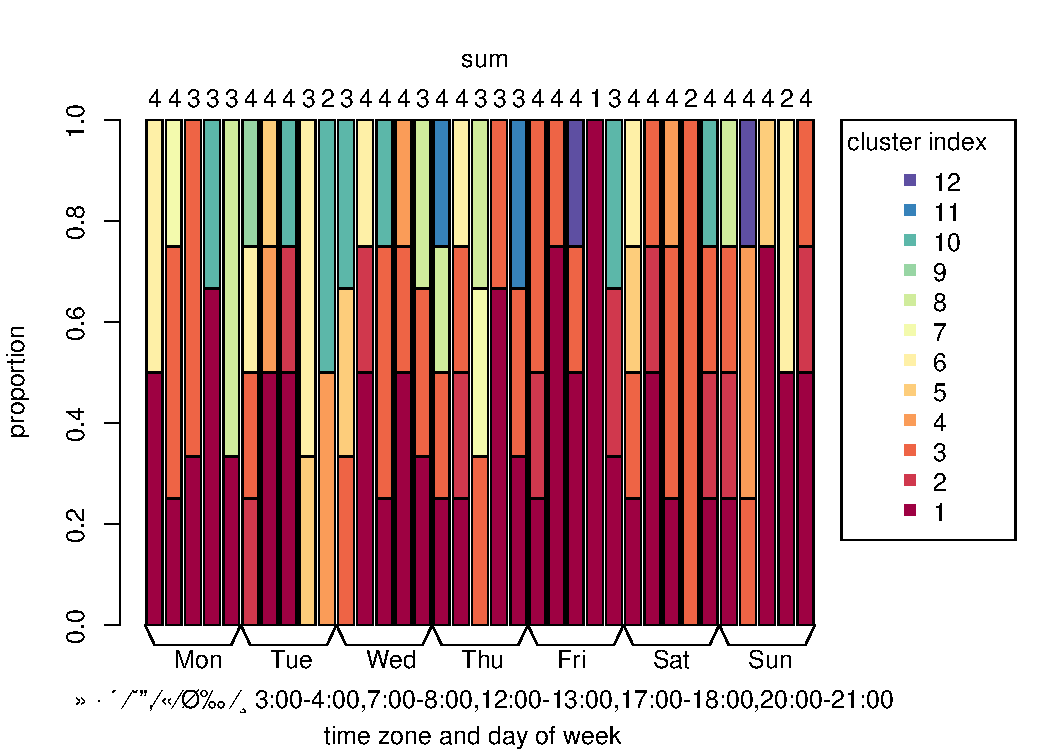
\includegraphics[height=3.5cm,width=5cm]{diff-eucl-ward-12-timezone-day.pdf}
}\\
\subfigure[クラスタ数 15 : 時間帯]{
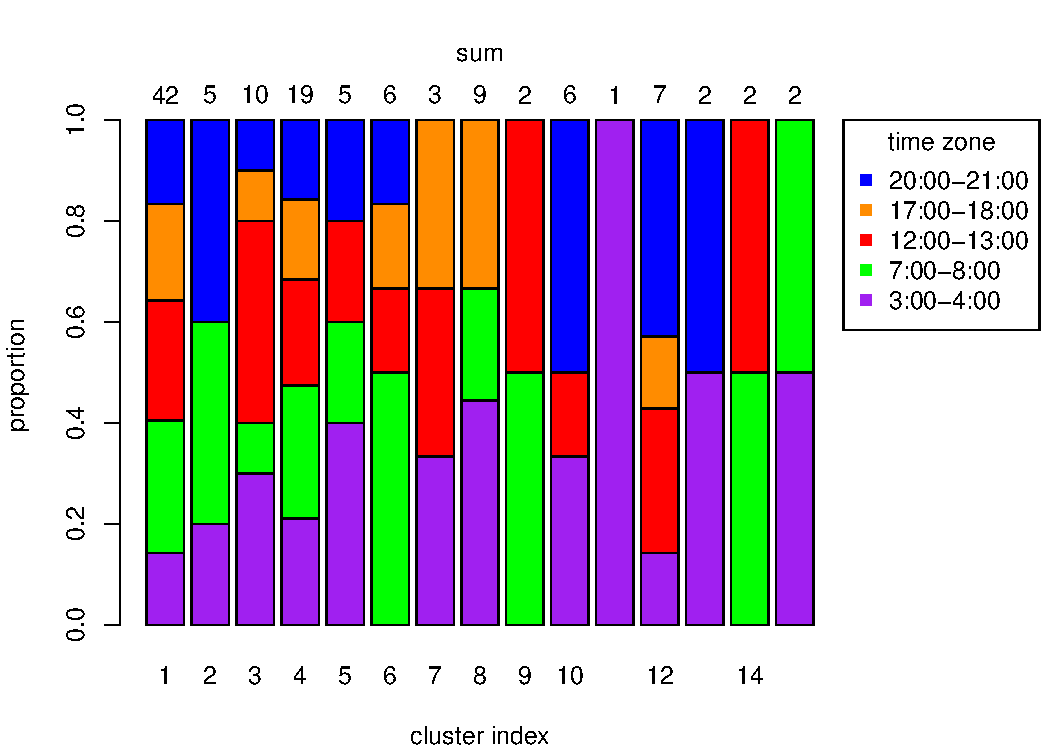
\includegraphics[height=3.5cm,width=5cm]{diff-eucl-ward-15-timezone.pdf}
}~
\subfigure[クラスタ数 15 : 曜日]{
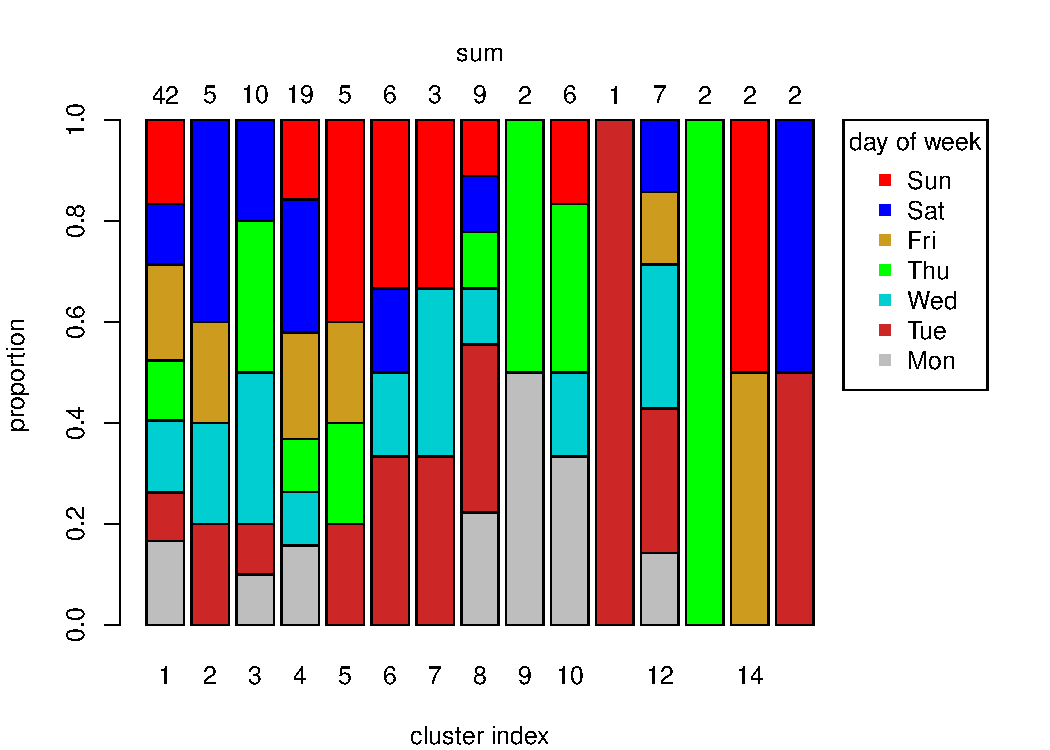
\includegraphics[height=3.5cm,width=5cm]{diff-eucl-ward-15-day.pdf}
}~
\subfigure[クラスタ数 15 : 時間帯と曜日]{
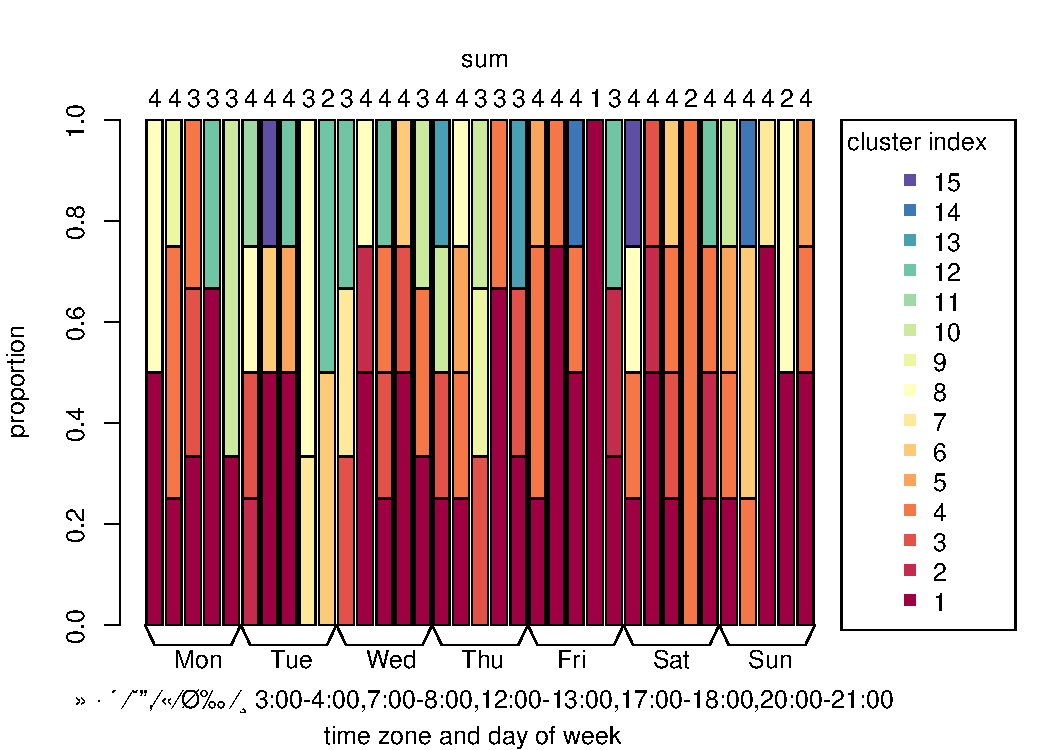
\includegraphics[height=3.5cm,width=5cm]{diff-eucl-ward-15-timezone-day.pdf}
}\\
\caption{AWS サーバを対象とした計測の変動値によるクラスタリング}
\end{center}
\end{figure}

\begin{figure}[tb]
\begin{center}
\subfigure[クラスタ数 6 : 時間帯]{
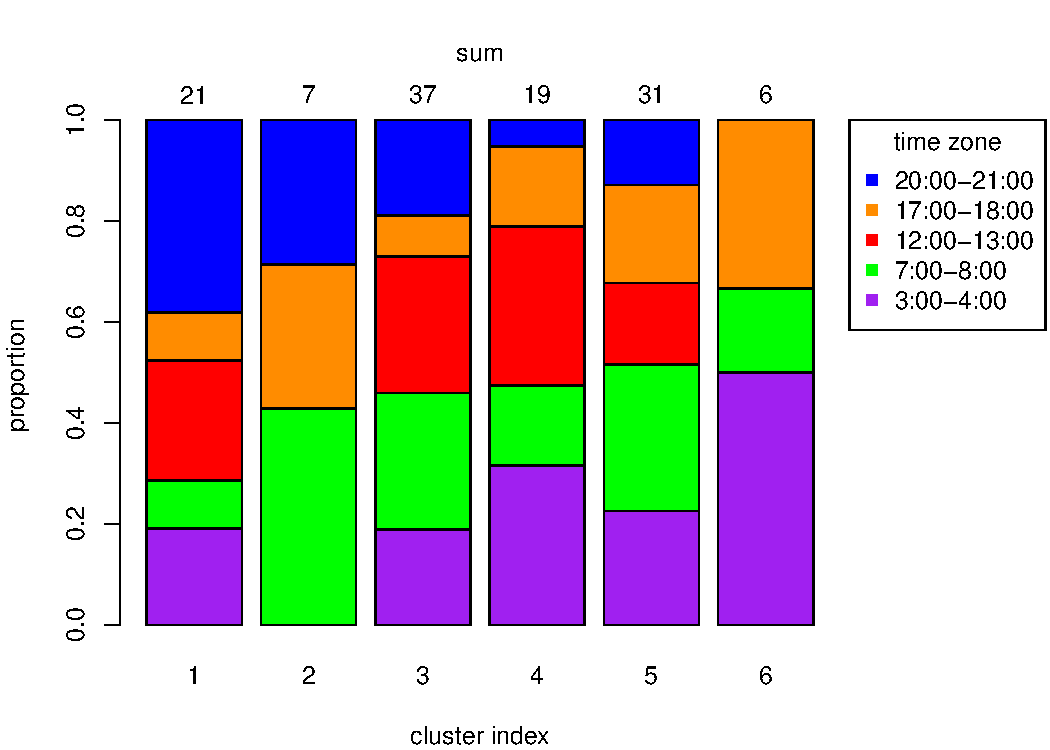
\includegraphics[height=3.5cm,width=5cm]{norm_comp-eucl-ward-6-timezone.pdf}
}~
\subfigure[クラスタ数 6 : 曜日]{
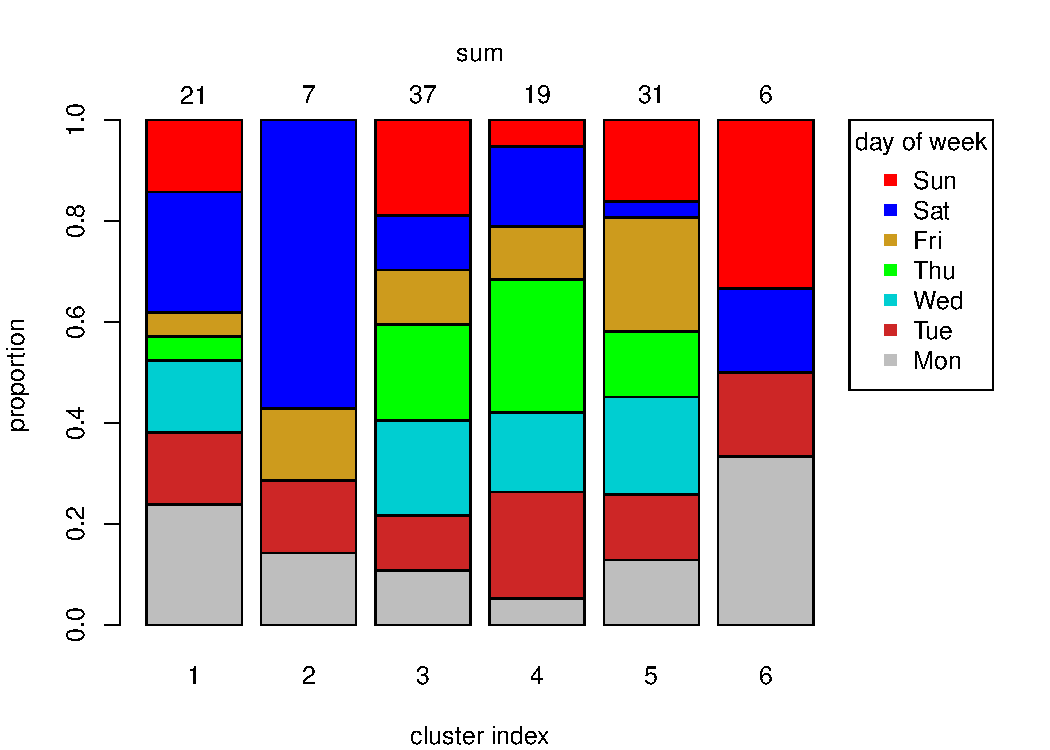
\includegraphics[height=3.5cm,width=5cm]{norm_comp-eucl-ward-6-day.pdf}
}~
\subfigure[クラスタ数 6 : 時間帯と曜日]{
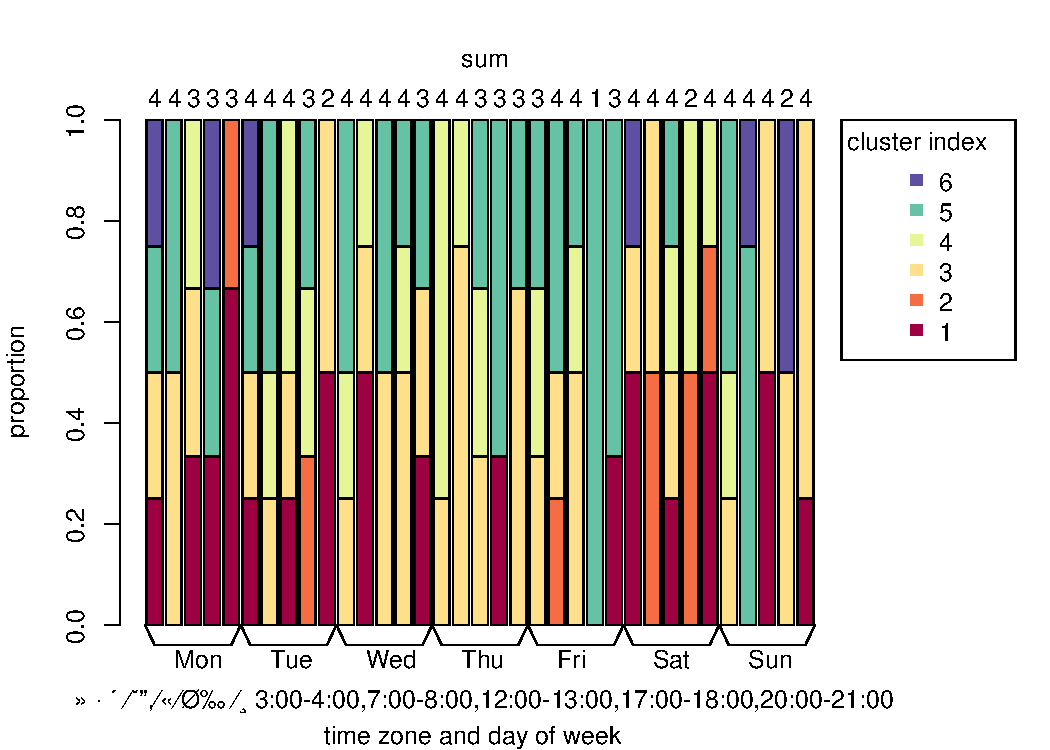
\includegraphics[height=3.5cm,width=5cm]{norm_comp-eucl-ward-6-timezone-day.pdf}
}\\
\subfigure[クラスタ数 7 : 時間帯]{
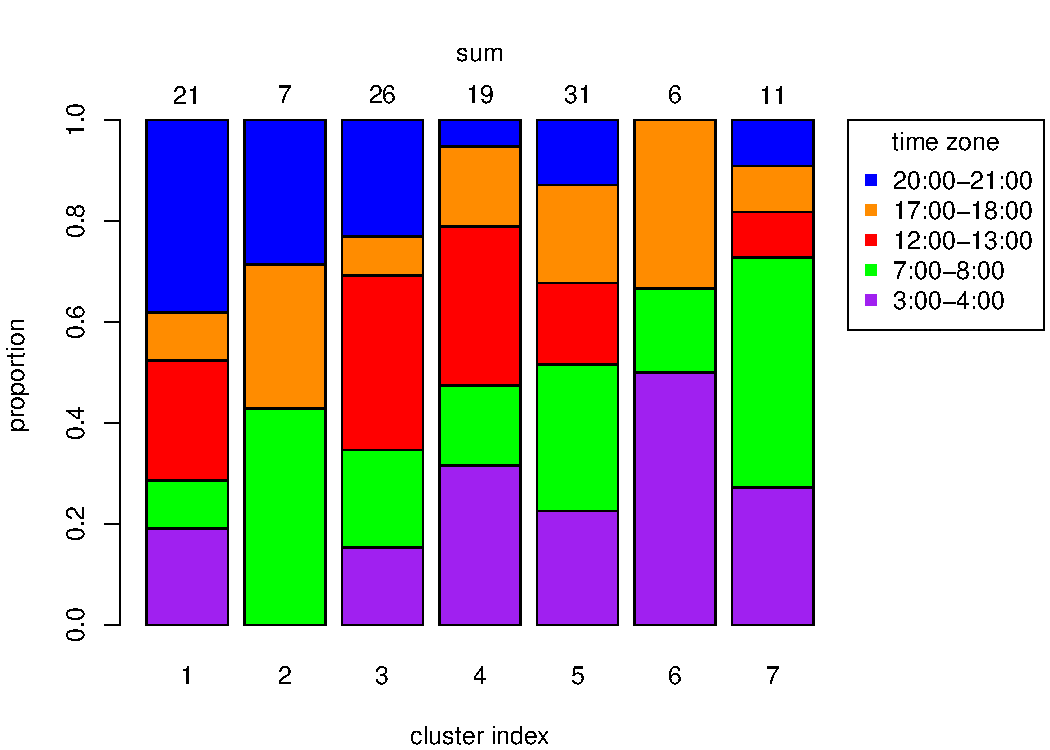
\includegraphics[height=3.5cm,width=5cm]{norm_comp-eucl-ward-7-timezone.pdf}
}~
\subfigure[クラスタ数 7 : 曜日]{
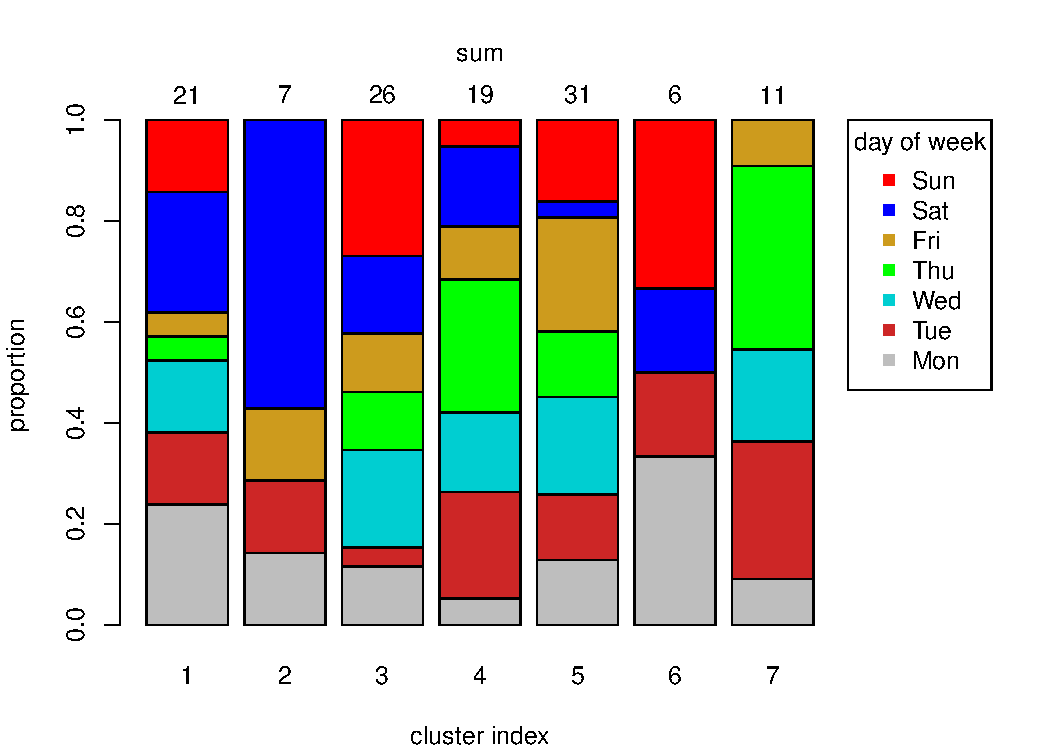
\includegraphics[height=3.5cm,width=5cm]{norm_comp-eucl-ward-7-day.pdf}
}~
\subfigure[クラスタ数 7 : 時間帯と曜日]{
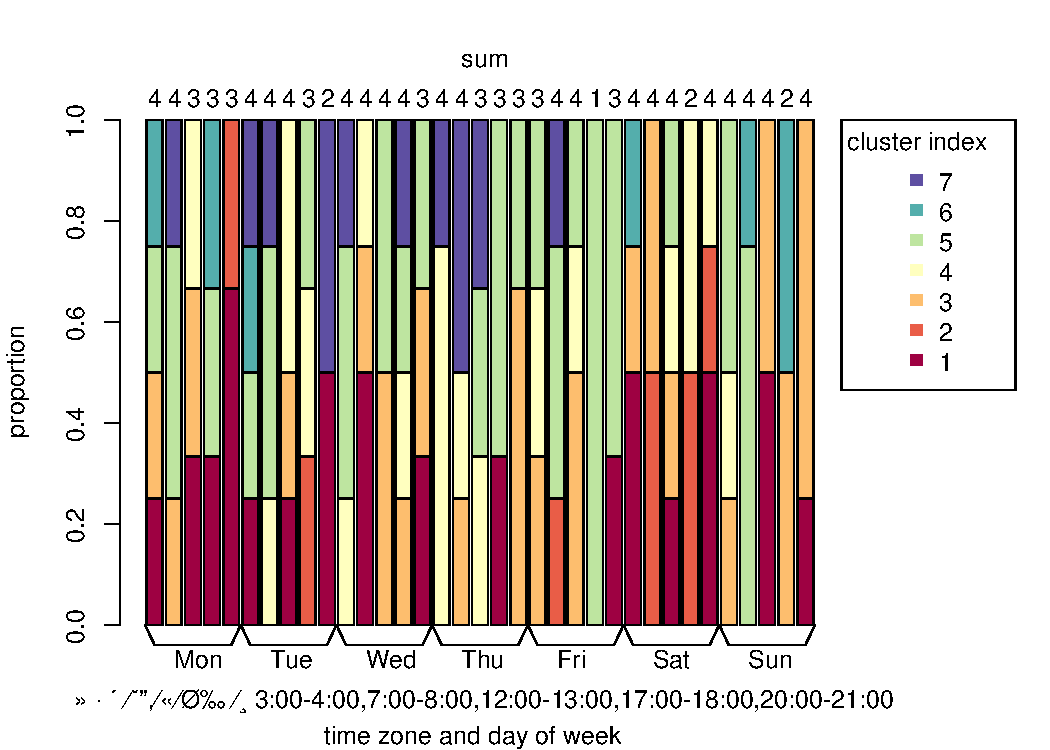
\includegraphics[height=3.5cm,width=5cm]{norm_comp-eucl-ward-7-timezone-day.pdf}
}\\
\subfigure[クラスタ数 9 : 時間帯]{
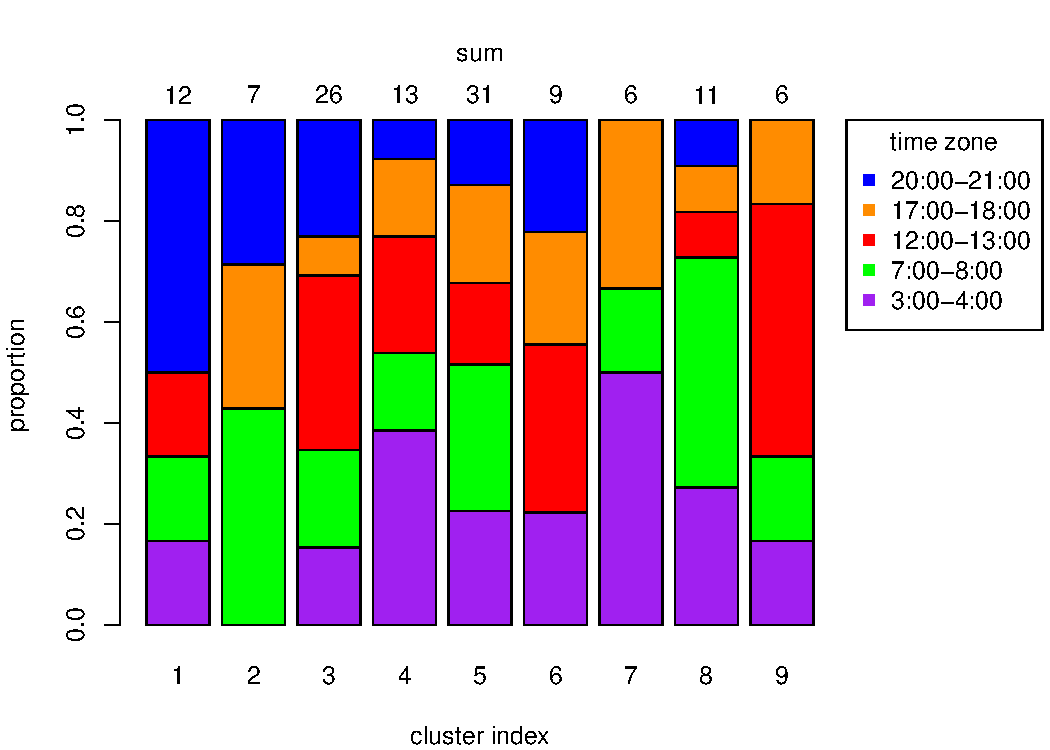
\includegraphics[height=3.5cm,width=5cm]{norm_comp-eucl-ward-9-timezone.pdf}
}~
\subfigure[クラスタ数 9 : 曜日]{
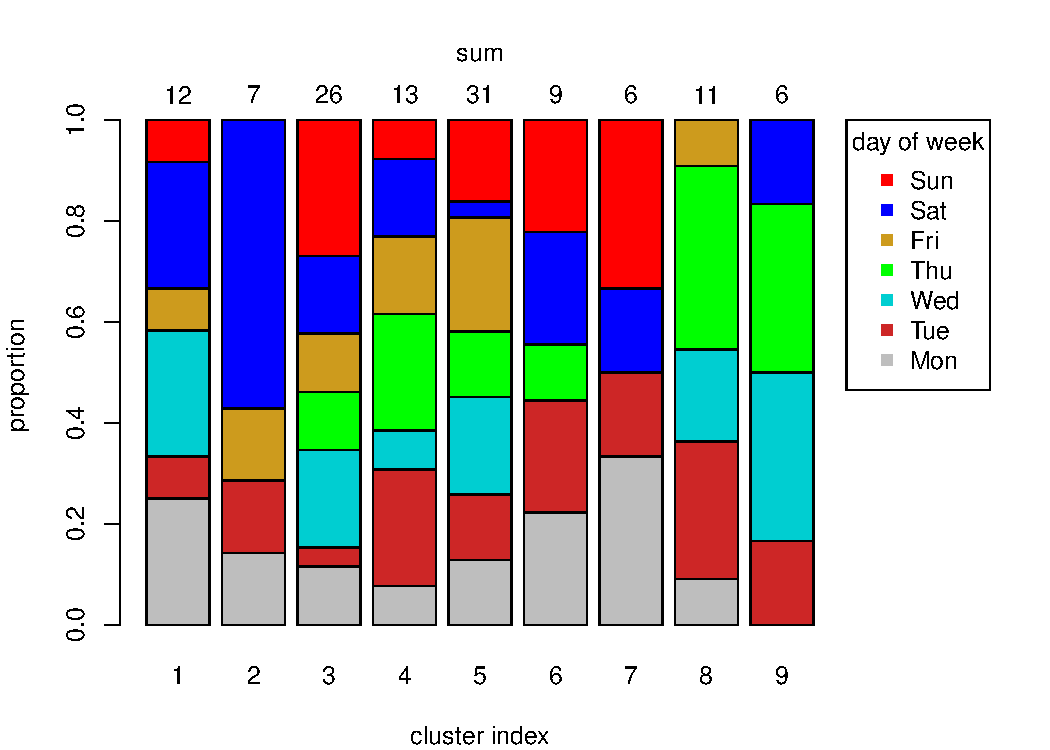
\includegraphics[height=3.5cm,width=5cm]{norm_comp-eucl-ward-9-day.pdf}
}~
\subfigure[クラスタ数 9 : 時間帯と曜日]{
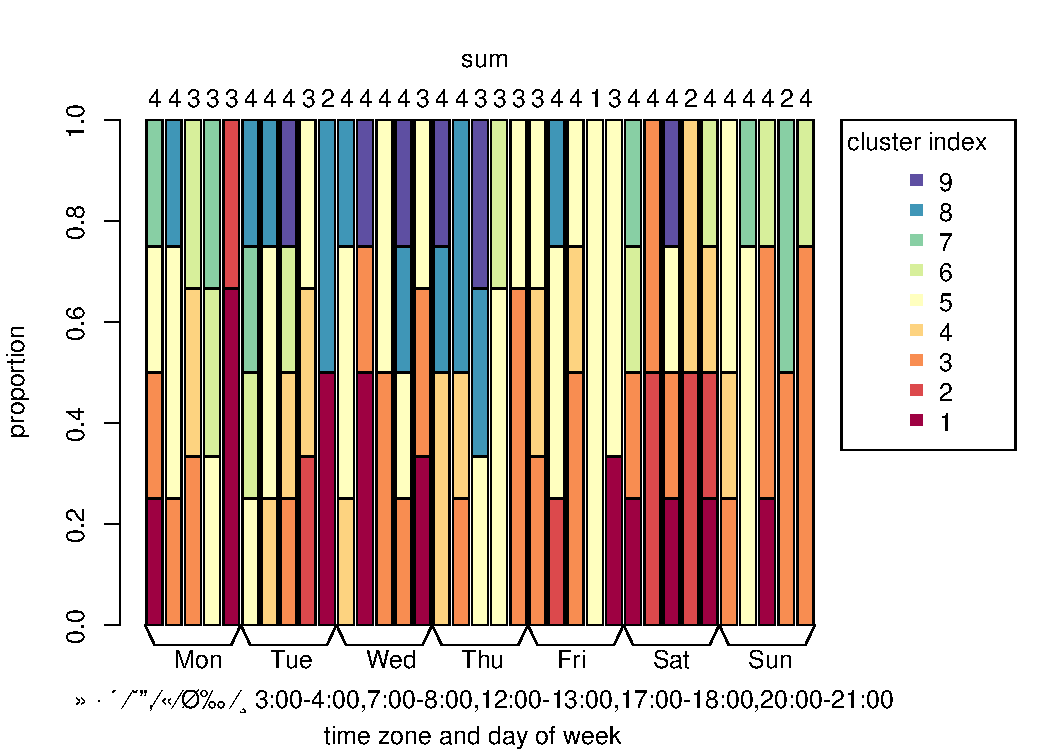
\includegraphics[height=3.5cm,width=5cm]{norm_comp-eucl-ward-9-timezone-day.pdf}
}\\
\subfigure[クラスタ数 12 : 時間帯]{
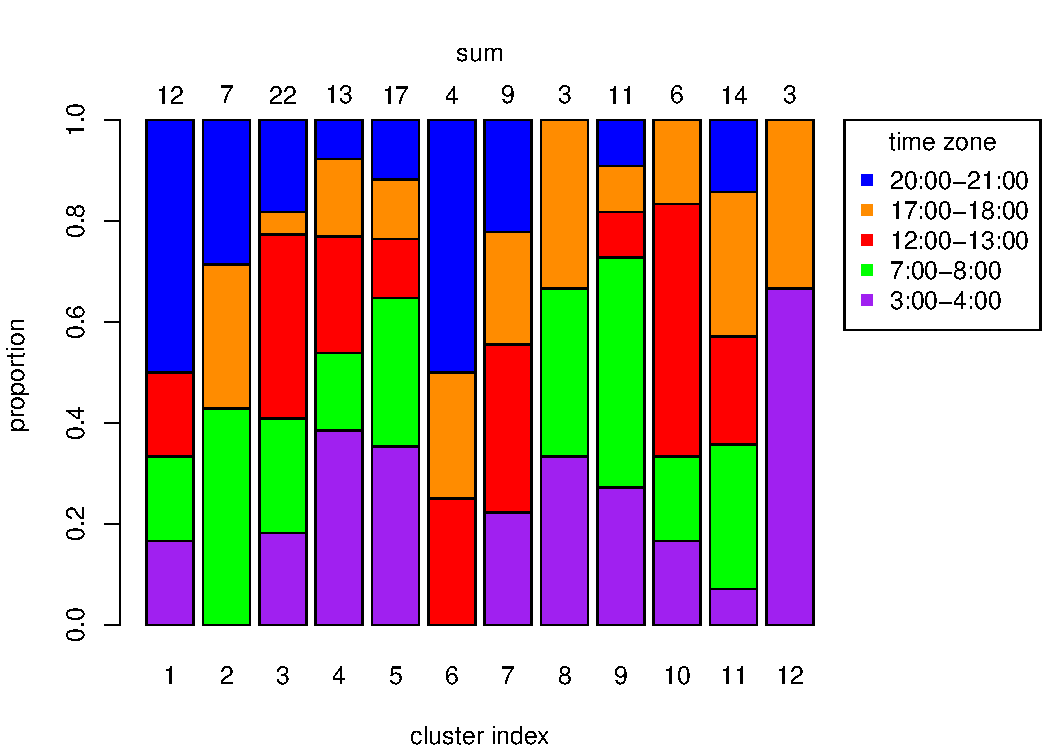
\includegraphics[height=3.5cm,width=5cm]{norm_comp-eucl-ward-12-timezone.pdf}
}~
\subfigure[クラスタ数 12 : 曜日]{
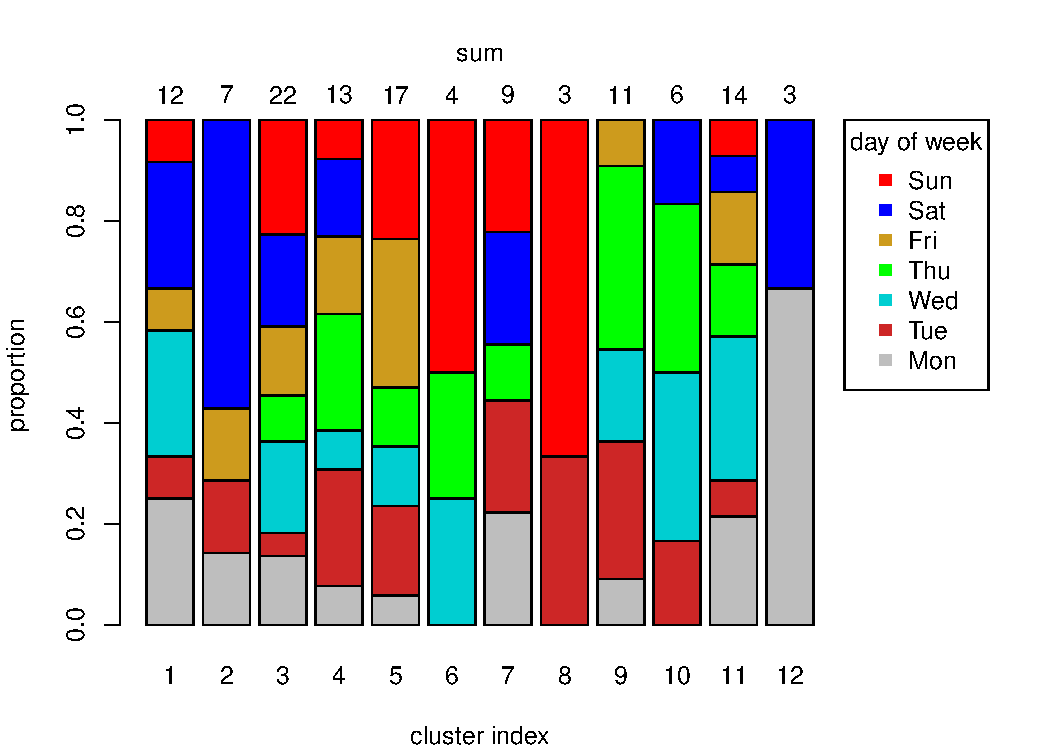
\includegraphics[height=3.5cm,width=5cm]{norm_comp-eucl-ward-12-day.pdf}
}~
\subfigure[クラスタ数 12 : 時間帯と曜日]{
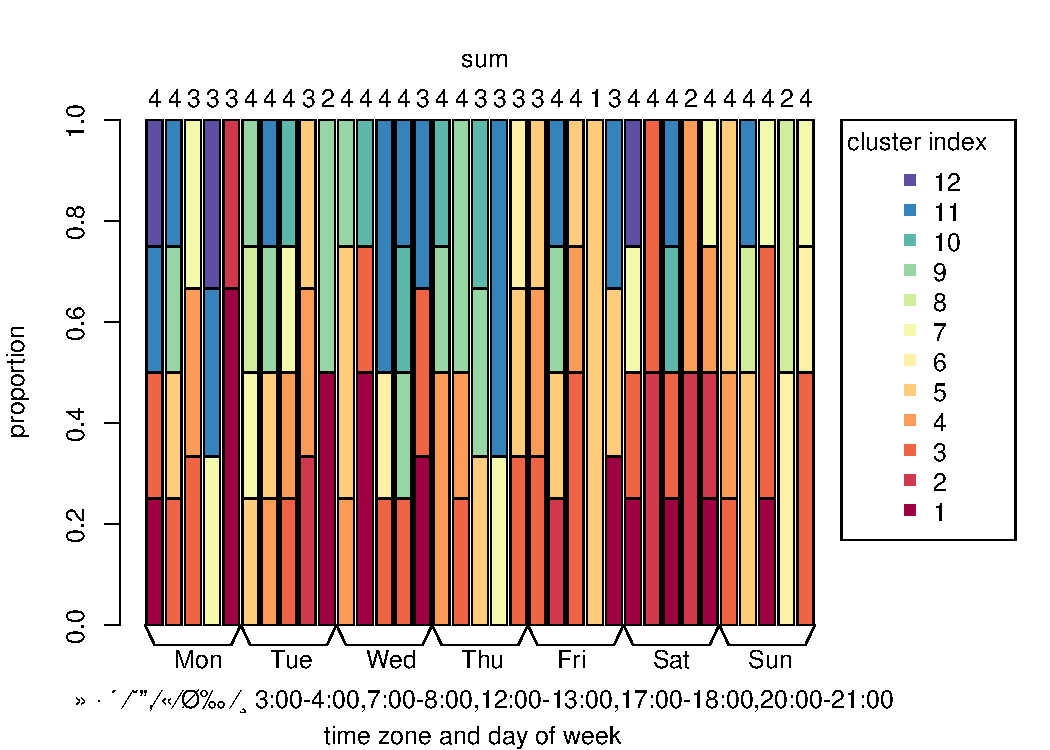
\includegraphics[height=3.5cm,width=5cm]{norm_comp-eucl-ward-12-timezone-day.pdf}
}\\
\subfigure[クラスタ数 15 : 時間帯]{
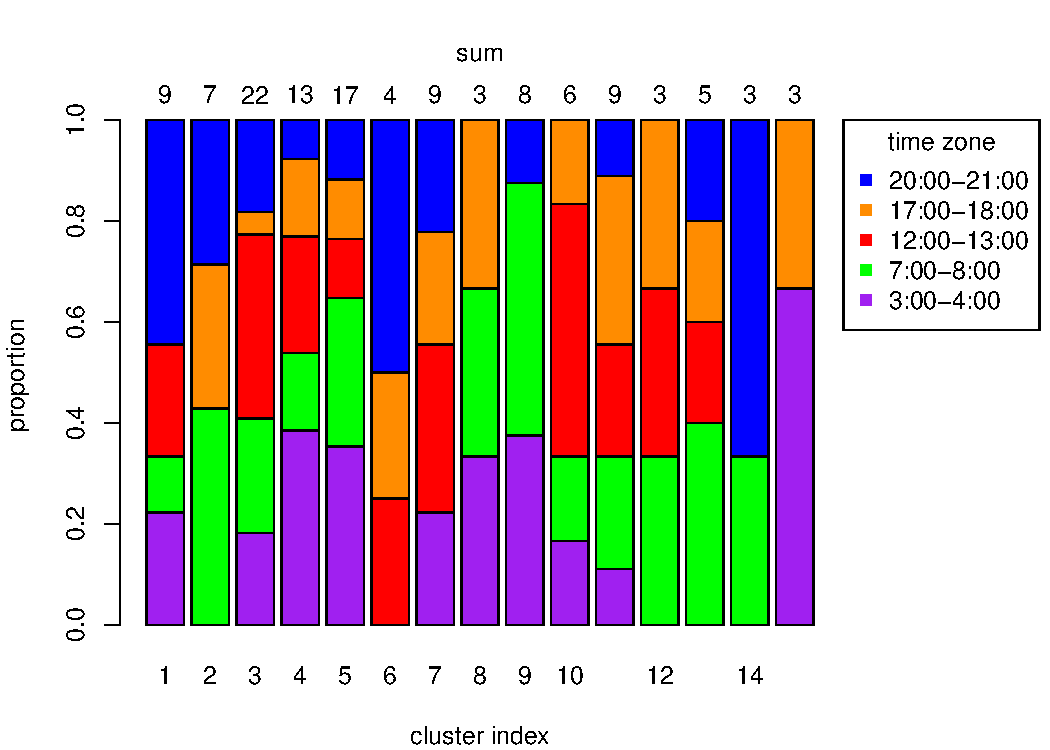
\includegraphics[height=3.5cm,width=5cm]{norm_comp-eucl-ward-15-timezone.pdf}
}~
\subfigure[クラスタ数 15 : 曜日]{
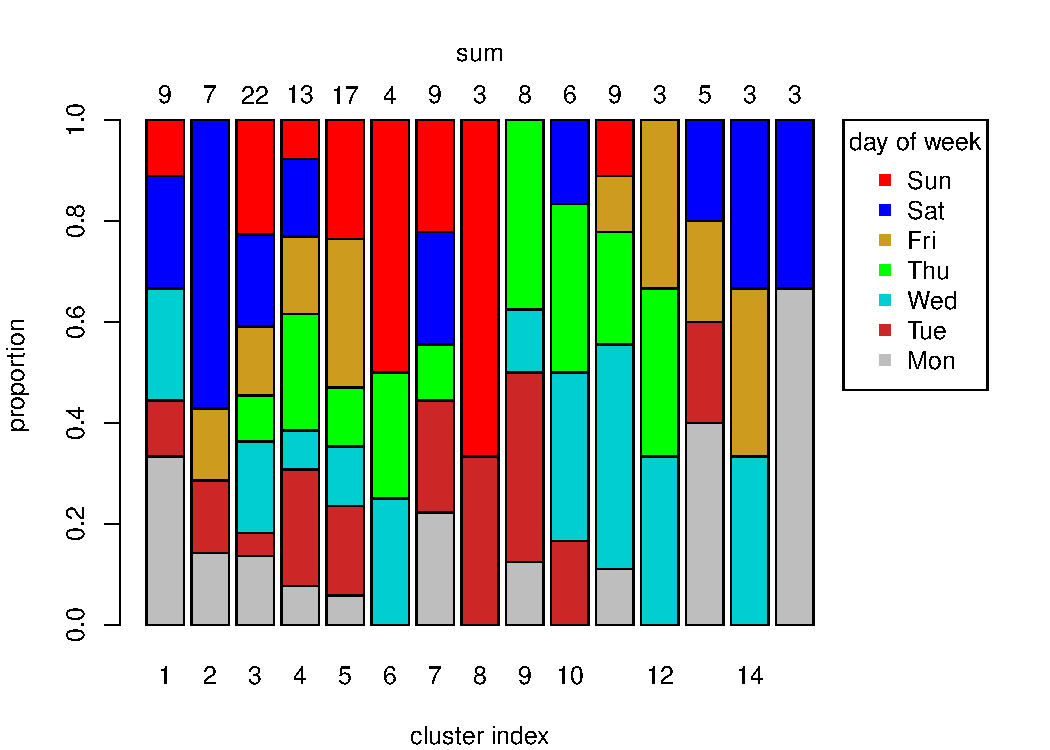
\includegraphics[height=3.5cm,width=5cm]{norm_comp-eucl-ward-15-day.pdf}
}~
\subfigure[クラスタ数 15 : 時間帯と曜日]{
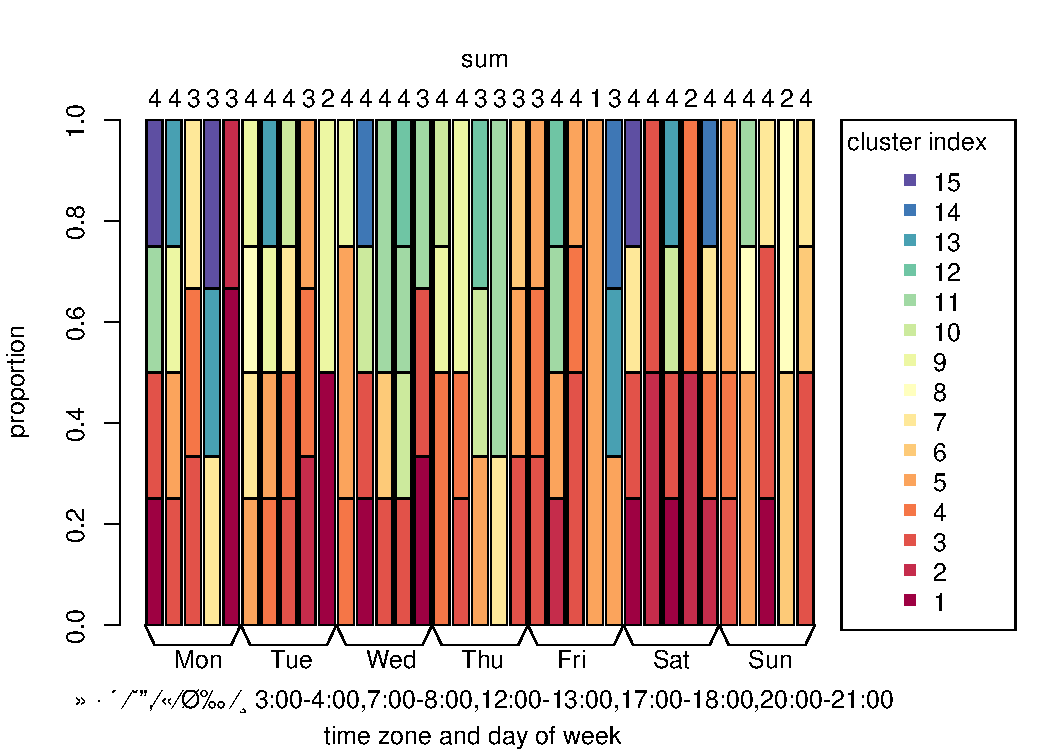
\includegraphics[height=3.5cm,width=5cm]{norm_comp-eucl-ward-15-timezone-day.pdf}
}\\
\caption{AWS サーバを対象とした計測の実測値の主成分によるクラスタリング}
\end{center}
\end{figure}

\begin{figure}[tb]
\begin{center}
\subfigure[クラスタ数 6 : 時間帯]{
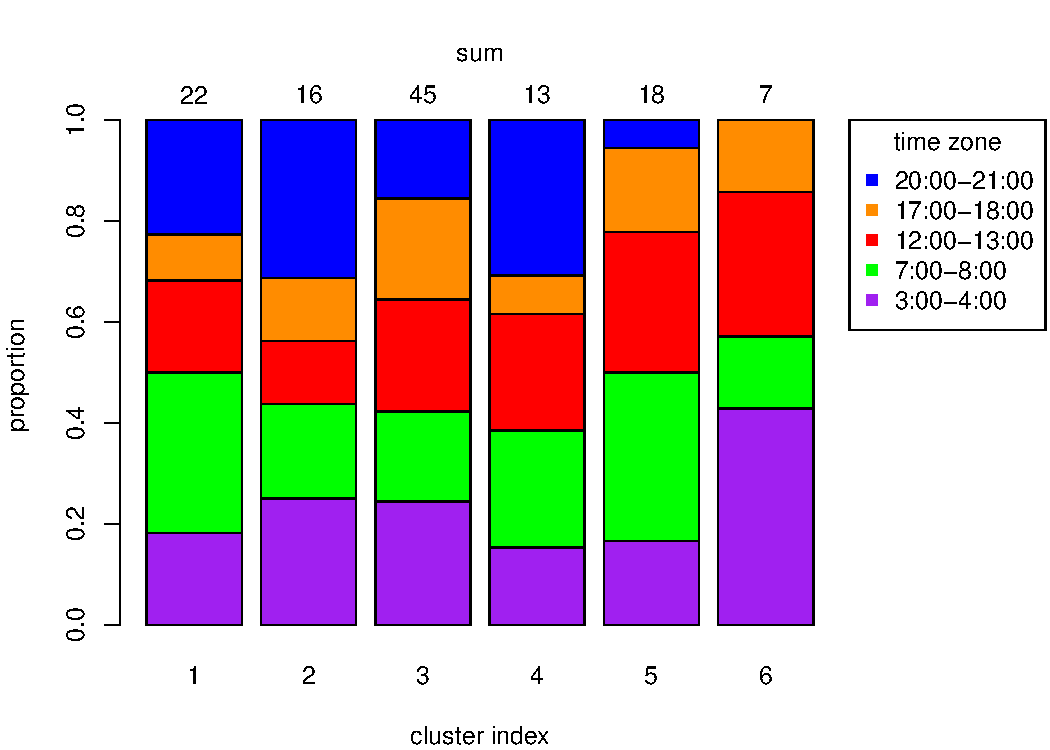
\includegraphics[height=3.5cm,width=5cm]{diff_comp-eucl-ward-6-timezone.pdf}
}~
\subfigure[クラスタ数 6 : 曜日]{
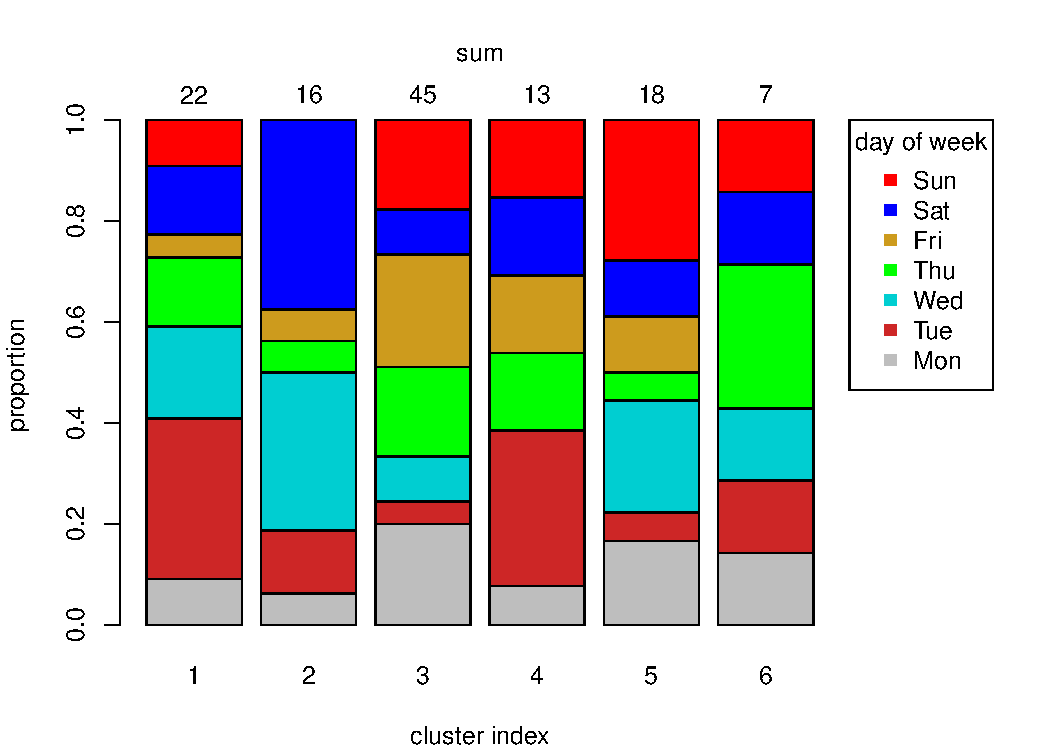
\includegraphics[height=3.5cm,width=5cm]{diff_comp-eucl-ward-6-day.pdf}
}~
\subfigure[クラスタ数 6 : 時間帯と曜日]{
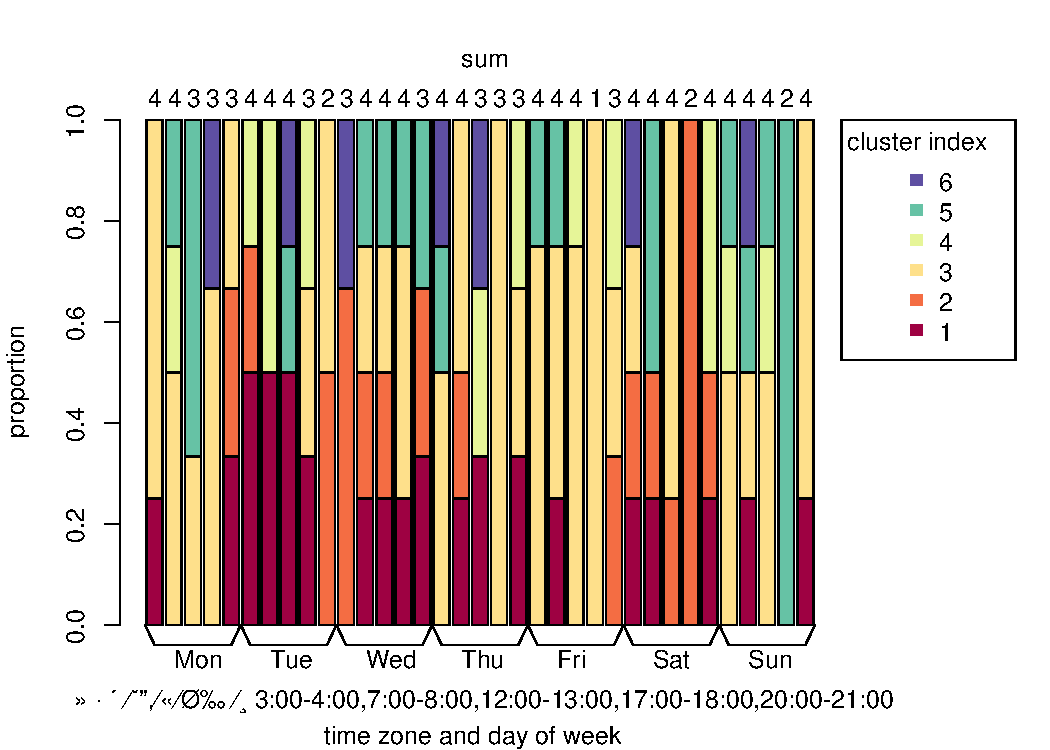
\includegraphics[height=3.5cm,width=5cm]{diff_comp-eucl-ward-6-timezone-day.pdf}
}\\
\subfigure[クラスタ数 7 : 時間帯]{
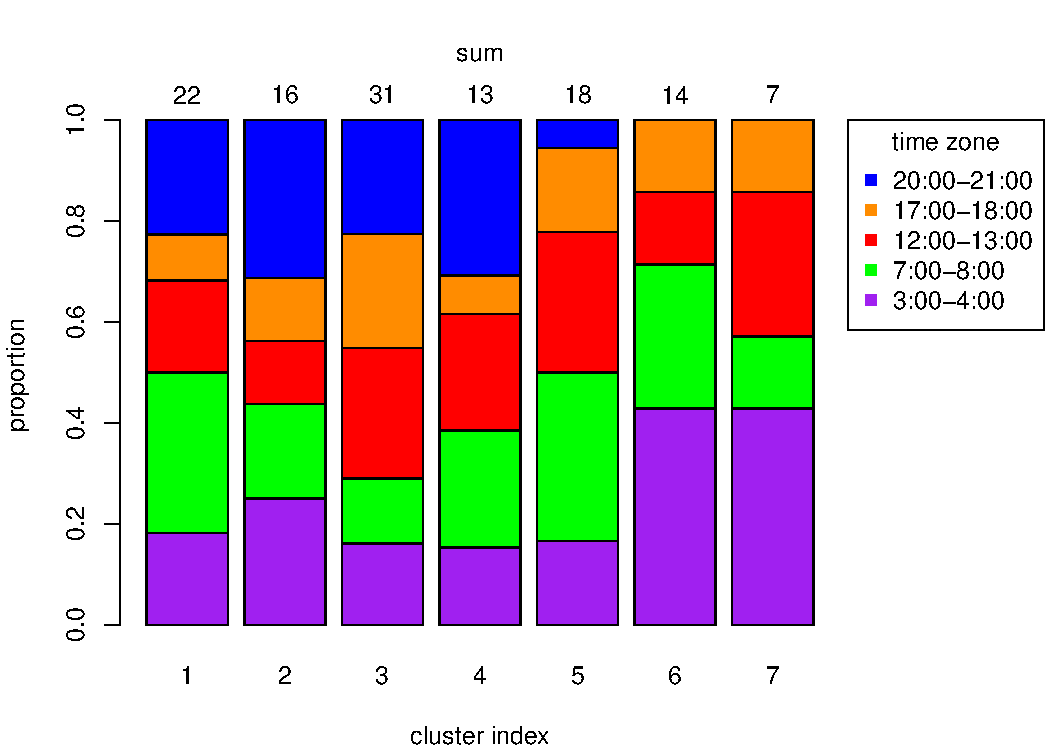
\includegraphics[height=3.5cm,width=5cm]{diff_comp-eucl-ward-7-timezone.pdf}
}~
\subfigure[クラスタ数 7 : 曜日]{
\includegraphics[height=3.5cm,width=5cm]{diff_comp-eucl-ward-7-day.pdf}
}~
\subfigure[クラスタ数 7 : 時間帯と曜日]{
\includegraphics[height=3.5cm,width=5cm]{diff_comp-eucl-ward-7-timezone-day.pdf}
}\\
\subfigure[クラスタ数 9 : 時間帯]{
\includegraphics[height=3.5cm,width=5cm]{diff_comp-eucl-ward-9-timezone.pdf}
}~
\subfigure[クラスタ数 9 : 曜日]{
\includegraphics[height=3.5cm,width=5cm]{diff_comp-eucl-ward-9-day.pdf}
}~
\subfigure[クラスタ数 9 : 時間帯と曜日]{
\includegraphics[height=3.5cm,width=5cm]{diff_comp-eucl-ward-9-timezone-day.pdf}
}\\
\subfigure[クラスタ数 12 : 時間帯]{
\includegraphics[height=3.5cm,width=5cm]{diff_comp-eucl-ward-12-timezone.pdf}
}~
\subfigure[クラスタ数 12 : 曜日]{
\includegraphics[height=3.5cm,width=5cm]{diff_comp-eucl-ward-12-day.pdf}
}~
\subfigure[クラスタ数 12 : 時間帯と曜日]{
\includegraphics[height=3.5cm,width=5cm]{diff_comp-eucl-ward-12-timezone-day.pdf}
}\\
\subfigure[クラスタ数 15 : 時間帯]{
\includegraphics[height=3.5cm,width=5cm]{diff_comp-eucl-ward-15-timezone.pdf}
}~
\subfigure[クラスタ数 15 : 曜日]{
\includegraphics[height=3.5cm,width=5cm]{diff_comp-eucl-ward-15-day.pdf}
}~
\subfigure[クラスタ数 15 : 時間帯と曜日]{
\includegraphics[height=3.5cm,width=5cm]{diff_comp-eucl-ward-15-timezone-day.pdf}
}\\
\caption{AWS サーバを対象とした計測の変動値の主成分によるクラスタリング}
\end{center}
\end{figure}


\begin{figure}[tb]
\begin{center}
\subfigure[クラスタ数 6 : 時間帯]{
\includegraphics[height=3.5cm,width=5cm]{norm-eucl-ward-6-timezone-sinet.pdf}
}~
\subfigure[クラスタ数 6 : 曜日]{
\includegraphics[height=3.5cm,width=5cm]{norm-eucl-ward-6-day-sinet.pdf}
}~
\subfigure[クラスタ数 6 : 時間帯と曜日]{
\includegraphics[height=3.5cm,width=5cm]{norm-eucl-ward-6-timezone-day-sinet.pdf}
}\\
\subfigure[クラスタ数 7 : 時間帯]{
\includegraphics[height=3.5cm,width=5cm]{norm-eucl-ward-7-timezone-sinet.pdf}
}~
\subfigure[クラスタ数 7 : 曜日]{
\includegraphics[height=3.5cm,width=5cm]{norm-eucl-ward-7-day-sinet.pdf}
}~
\subfigure[クラスタ数 7 : 時間帯と曜日]{
\includegraphics[height=3.5cm,width=5cm]{norm-eucl-ward-7-timezone-day-sinet.pdf}
}\\
\subfigure[クラスタ数 9 : 時間帯]{
\includegraphics[height=3.5cm,width=5cm]{norm-eucl-ward-9-timezone-sinet.pdf}
}~
\subfigure[クラスタ数 9 : 曜日]{
\includegraphics[height=3.5cm,width=5cm]{norm-eucl-ward-9-day-sinet.pdf}
}~
\subfigure[クラスタ数 9 : 時間帯と曜日]{
\includegraphics[height=3.5cm,width=5cm]{norm-eucl-ward-9-timezone-day-sinet.pdf}
}\\
\subfigure[クラスタ数 12 : 時間帯]{
\includegraphics[height=3.5cm,width=5cm]{norm-eucl-ward-12-timezone-sinet.pdf}
}~
\subfigure[クラスタ数 12 : 曜日]{
\includegraphics[height=3.5cm,width=5cm]{norm-eucl-ward-12-day-sinet.pdf}
}~
\subfigure[クラスタ数 12 : 時間帯と曜日]{
\includegraphics[height=3.5cm,width=5cm]{norm-eucl-ward-12-timezone-day-sinet.pdf}
}\\
\subfigure[クラスタ数 15 : 時間帯]{
\includegraphics[height=3.5cm,width=5cm]{norm-eucl-ward-15-timezone-sinet.pdf}
}~
\subfigure[クラスタ数 15 : 曜日]{
\includegraphics[height=3.5cm,width=5cm]{norm-eucl-ward-15-day-sinet.pdf}
}~
\subfigure[クラスタ数 15 : 時間帯と曜日]{
\includegraphics[height=3.5cm,width=5cm]{norm-eucl-ward-15-timezone-day-sinet.pdf}
}\\
\caption{SINET のウェブサーバを対象とした計測の実測値によるクラスタリング}
\label{cluster1}
\end{center}
\end{figure}

\begin{figure}[tb]
\begin{center}
\subfigure[クラスタ数 6 : 時間帯]{
\includegraphics[height=3.5cm,width=5cm]{diff-eucl-ward-6-timezone-sinet.pdf}
}~
\subfigure[クラスタ数 6 : 曜日]{
\includegraphics[height=3.5cm,width=5cm]{diff-eucl-ward-6-day-sinet.pdf}
}~
\subfigure[クラスタ数 6 : 時間帯と曜日]{
\includegraphics[height=3.5cm,width=5cm]{diff-eucl-ward-6-timezone-day-sinet.pdf}
}\\
\subfigure[クラスタ数 7 : 時間帯]{
\includegraphics[height=3.5cm,width=5cm]{diff-eucl-ward-7-timezone-sinet.pdf}
}~
\subfigure[クラスタ数 7 : 曜日]{
\includegraphics[height=3.5cm,width=5cm]{diff-eucl-ward-7-day-sinet.pdf}
}~
\subfigure[クラスタ数 7 : 時間帯と曜日]{
\includegraphics[height=3.5cm,width=5cm]{diff-eucl-ward-7-timezone-day-sinet.pdf}
}\\
\subfigure[クラスタ数 9 : 時間帯]{
\includegraphics[height=3.5cm,width=5cm]{diff-eucl-ward-9-timezone-sinet.pdf}
}~
\subfigure[クラスタ数 9 : 曜日]{
\includegraphics[height=3.5cm,width=5cm]{diff-eucl-ward-9-day-sinet.pdf}
}~
\subfigure[クラスタ数 9 : 時間帯と曜日]{
\includegraphics[height=3.5cm,width=5cm]{diff-eucl-ward-9-timezone-day-sinet.pdf}
}\\
\subfigure[クラスタ数 12 : 時間帯]{
\includegraphics[height=3.5cm,width=5cm]{diff-eucl-ward-12-timezone-sinet.pdf}
}~
\subfigure[クラスタ数 12 : 曜日]{
\includegraphics[height=3.5cm,width=5cm]{diff-eucl-ward-12-day-sinet.pdf}
}~
\subfigure[クラスタ数 12 : 時間帯と曜日]{
\includegraphics[height=3.5cm,width=5cm]{diff-eucl-ward-12-timezone-day-sinet.pdf}
}\\
\subfigure[クラスタ数 15 : 時間帯]{
\includegraphics[height=3.5cm,width=5cm]{diff-eucl-ward-15-timezone-sinet.pdf}
}~
\subfigure[クラスタ数 15 : 曜日]{
\includegraphics[height=3.5cm,width=5cm]{diff-eucl-ward-15-day-sinet.pdf}
}~
\subfigure[クラスタ数 15 : 時間帯と曜日]{
\includegraphics[height=3.5cm,width=5cm]{diff-eucl-ward-15-timezone-day-sinet.pdf}
}\\
\caption{SINET のウェブサーバを対象とした計測の変動値によるクラスタリング}
\end{center}
\end{figure}

\begin{figure}[tb]
\begin{center}
\subfigure[クラスタ数 6 : 時間帯]{
\includegraphics[height=3.5cm,width=5cm]{norm_comp-eucl-ward-6-timezone-sinet.pdf}
}~
\subfigure[クラスタ数 6 : 曜日]{
\includegraphics[height=3.5cm,width=5cm]{norm_comp-eucl-ward-6-day-sinet.pdf}
}~
\subfigure[クラスタ数 6 : 時間帯と曜日]{
\includegraphics[height=3.5cm,width=5cm]{norm_comp-eucl-ward-6-timezone-day-sinet.pdf}
}\\
\subfigure[クラスタ数 7 : 時間帯]{
\includegraphics[height=3.5cm,width=5cm]{norm_comp-eucl-ward-7-timezone-sinet.pdf}
}~
\subfigure[クラスタ数 7 : 曜日]{
\includegraphics[height=3.5cm,width=5cm]{norm_comp-eucl-ward-7-day-sinet.pdf}
}~
\subfigure[クラスタ数 7 : 時間帯と曜日]{
\includegraphics[height=3.5cm,width=5cm]{norm_comp-eucl-ward-7-timezone-day-sinet.pdf}
}\\
\subfigure[クラスタ数 9 : 時間帯]{
\includegraphics[height=3.5cm,width=5cm]{norm_comp-eucl-ward-9-timezone-sinet.pdf}
}~
\subfigure[クラスタ数 9 : 曜日]{
\includegraphics[height=3.5cm,width=5cm]{norm_comp-eucl-ward-9-day-sinet.pdf}
}~
\subfigure[クラスタ数 9 : 時間帯と曜日]{
\includegraphics[height=3.5cm,width=5cm]{norm_comp-eucl-ward-9-timezone-day-sinet.pdf}
}\\
\subfigure[クラスタ数 12 : 時間帯]{
\includegraphics[height=3.5cm,width=5cm]{norm_comp-eucl-ward-12-timezone-sinet.pdf}
}~
\subfigure[クラスタ数 12 : 曜日]{
\includegraphics[height=3.5cm,width=5cm]{norm_comp-eucl-ward-12-day-sinet.pdf}
}~
\subfigure[クラスタ数 12 : 時間帯と曜日]{
\includegraphics[height=3.5cm,width=5cm]{norm_comp-eucl-ward-12-timezone-day-sinet.pdf}
}\\
\subfigure[クラスタ数 15 : 時間帯]{
\includegraphics[height=3.5cm,width=5cm]{norm_comp-eucl-ward-15-timezone-sinet.pdf}
}~
\subfigure[クラスタ数 15 : 曜日]{
\includegraphics[height=3.5cm,width=5cm]{norm_comp-eucl-ward-15-day-sinet.pdf}
}~
\subfigure[クラスタ数 15 : 時間帯と曜日]{
\includegraphics[height=3.5cm,width=5cm]{norm_comp-eucl-ward-15-timezone-day-sinet.pdf}
}\\
\caption{SINET のウェブサーバを対象とした計測の実測値の主成分によるクラスタリング}
\end{center}
\end{figure}

\begin{figure}[tb]
\begin{center}
\subfigure[クラスタ数 6 : 時間帯]{
\includegraphics[height=3.5cm,width=5cm]{diff_comp-eucl-ward-6-timezone-sinet.pdf}
}~
\subfigure[クラスタ数 6 : 曜日]{
\includegraphics[height=3.5cm,width=5cm]{diff_comp-eucl-ward-6-day-sinet.pdf}
}~
\subfigure[クラスタ数 6 : 時間帯と曜日]{
\includegraphics[height=3.5cm,width=5cm]{diff_comp-eucl-ward-6-timezone-day-sinet.pdf}
}\\
\subfigure[クラスタ数 7 : 時間帯]{
\includegraphics[height=3.5cm,width=5cm]{diff_comp-eucl-ward-7-timezone-sinet.pdf}
}~
\subfigure[クラスタ数 7 : 曜日]{
\includegraphics[height=3.5cm,width=5cm]{diff_comp-eucl-ward-7-day-sinet.pdf}
}~
\subfigure[クラスタ数 7 : 時間帯と曜日]{
\includegraphics[height=3.5cm,width=5cm]{diff_comp-eucl-ward-7-timezone-day-sinet.pdf}
}\\
\subfigure[クラスタ数 9 : 時間帯]{
\includegraphics[height=3.5cm,width=5cm]{diff_comp-eucl-ward-9-timezone-sinet.pdf}
}~
\subfigure[クラスタ数 9 : 曜日]{
\includegraphics[height=3.5cm,width=5cm]{diff_comp-eucl-ward-9-day-sinet.pdf}
}~
\subfigure[クラスタ数 9 : 時間帯と曜日]{
\includegraphics[height=3.5cm,width=5cm]{diff_comp-eucl-ward-9-timezone-day-sinet.pdf}
}\\
\subfigure[クラスタ数 12 : 時間帯]{
\includegraphics[height=3.5cm,width=5cm]{diff_comp-eucl-ward-12-timezone-sinet.pdf}
}~
\subfigure[クラスタ数 12 : 曜日]{
\includegraphics[height=3.5cm,width=5cm]{diff_comp-eucl-ward-12-day-sinet.pdf}
}~
\subfigure[クラスタ数 12 : 時間帯と曜日]{
\includegraphics[height=3.5cm,width=5cm]{diff_comp-eucl-ward-12-timezone-day-sinet.pdf}
}\\
\subfigure[クラスタ数 15 : 時間帯]{
\includegraphics[height=3.5cm,width=5cm]{diff_comp-eucl-ward-15-timezone-sinet.pdf}
}~
\subfigure[クラスタ数 15 : 曜日]{
\includegraphics[height=3.5cm,width=5cm]{diff_comp-eucl-ward-15-day-sinet.pdf}
}~
\subfigure[クラスタ数 15 : 時間帯と曜日]{
\includegraphics[height=3.5cm,width=5cm]{diff_comp-eucl-ward-15-timezone-day-sinet.pdf}
}\\
\caption{SINET のウェブサーバを対象とした計測の変動値の主成分によるクラスタリング}
\label{cluster-2}
\end{center}
\end{figure}

\section{エルボー法による最適クラスタ数の決定}
エルボー法を用いて各データセットとそれに対する各クラスタリング手法における最適クラスタ数を定める.
各データセットは AWS サーバを対象とした計測で得られた実測値と変動値を ARMA-GARCH (2,2,1,1) で回帰したときのパラメータとその標準化後の主成分の計四つである.
クラスタリング手法は非階層的クラスタリングとして k 平均法の距離関数がユークリッド距離,階層的クラスタリングとしてウォード法,最近傍法,重心法のそれぞれに対して距離関数がユークリッド距離,キャンベラ距離,マンハッタン距離とした計十個である.
要素 $\vector{w_i} = [w_{i1},w_{i2},...,w_{in}]$ として,
\begin{itemize}
\item ユークリッド距離 : $\sqrt{( \vector{w_i} - \vector{w_j} )^2}$
\item マンハッタン距離 : $\sum^n_{k=1} |w_{ik}-w_{jk}| $
\item キャンベラ距離 : $\sum^n_{k=1}\frac{|w_{ik}-w_{jk}|}{|w_{ik}|+|w_{jk}|} $
\end{itemize}

また,
\begin{itemize}
\item 重心法 : クラスタ間の重心距離が最小のクラスタ同士を融合する
\item 最近傍法 : クラスタ間の要素対のうち,最も近い要素間をクラスタ間距離として,クラスタ間距離が最も小さいクラスタ同士を融合する
\item ウォード法 : 融合後のクラスタ内分散から融合前の二つのクラスタ内分散の差を最小とするという基準でクラスタを融合する
\end{itemize}

ここでエルボー法とは,クラスタ内誤差分散(SSE : Sum of Squared errors of prediction)と呼ばれるクラスタの集約度をその小ささで表す指標を用いる.
クラスタ数を 1 から順に増やしていきながら逐次 SSE を算出し,最適クラスタ数を次のクラスタ数での SSE の変化の割合に対するそのクラスタ数での変化の割合を最大とする箇所と定める.
クラスタ数 $k$ での SSE は式 (\ref{sse}) で定められ,最適クラスタ数は式 (\ref{bestk}) となる.
ここでは,$2 \leq k \leq 15$ とした.
また,要素 $\vector{w_i}$ が属するクラスタ重心を $\vector{w_G}(\vector{w_i})$ とし,$dist(\vector{w_i},\vector{w_j})$ はそのクラスタリング手法における距離関数上での $\vector{w_i}$ と $\vector{w_j}$ の距離である.
\begin{equation}
SSE_k = \sum_i dist(\vector{w_i},\vector{w_G}(\vector{w_i}))^2
\label{sse}
\end{equation}
\begin{equation}
最適クラスタ数 = \argmax_{2 \leq k \leq 15} \frac{SSE_k - SSE_{k-1}}{SSE_{k+1} - SSE_k}
\label{bestk}
\end{equation}

以下の図は,各データセットと各クラスタリングにおいて,横軸をクラスタ数,縦軸を SSE でとったものを青線の折れ線グラフで示し,赤色の破線の箇所が最適クラスタ数の位置を示している.
また,その右図にはクラスタ数を最適クラスタ数としたときのクラスタリングにおける主成分散布図である.

\begin{figure}[tb]
\begin{center}
\subfigure[ウォード法,ユークリッド距離]{
\includegraphics[height=3.5cm,width=6.5cm]{norm-eucl-ward-sse.pdf}
}~
\subfigure[主成分散布図]{
\includegraphics[height=3.5cm,width=6.5cm]{norm-eucl-ward-compscat.pdf}
}\\
\subfigure[ウォード法,マンハッタン距離]{
\includegraphics[height=3.5cm,width=6.5cm]{norm-manh-ward-sse.pdf}
}~
\subfigure[主成分散布図]{
\includegraphics[height=3.5cm,width=6.5cm]{norm-manh-ward-compscat.pdf}
}\\
\subfigure[ウォード法,キャンベラ距離]{
\includegraphics[height=3.5cm,width=6.5cm]{norm-canb-ward-sse.pdf}
}~
\subfigure[主成分散布図]{
\includegraphics[height=3.5cm,width=6.5cm]{norm-canb-ward-compscat.pdf}
}\\
\subfigure[最近傍法,ユークリッド距離]{
\includegraphics[height=3.5cm,width=6.5cm]{norm-eucl-sing-sse.pdf}
}~
\subfigure[主成分散布図]{
\includegraphics[height=3.5cm,width=6.5cm]{norm-eucl-sing-compscat.pdf}
}\\
\subfigure[最近傍法,マンハッタン距離]{
\includegraphics[height=3.5cm,width=6.5cm]{norm-manh-sing-sse.pdf}
}~
\subfigure[主成分散布図]{
\includegraphics[height=3.5cm,width=6.5cm]{norm-manh-sing-compscat.pdf}
}\\
\caption{実測値によるクラスタリング}
\end{center}
\end{figure}
\begin{figure}[tb]
\begin{center}
\subfigure[最近傍法,キャンベラ距離]{
\includegraphics[height=3.5cm,width=6.5cm]{norm-canb-sing-sse.pdf}
}~
\subfigure[主成分散布図]{
\includegraphics[height=3.5cm,width=6.5cm]{norm-canb-sing-compscat.pdf}
}\\
\subfigure[重心法,ユークリッド距離]{
\includegraphics[height=3.5cm,width=6.5cm]{norm-eucl-cent-sse.pdf}
}~
\subfigure[主成分散布図]{
\includegraphics[height=3.5cm,width=6.5cm]{norm-eucl-cent-compscat.pdf}
}\\
\subfigure[重心法,マンハッタン距離]{
\includegraphics[height=3.5cm,width=6.5cm]{norm-manh-cent-sse.pdf}
}~
\subfigure[主成分散布図]{
\includegraphics[height=3.5cm,width=6.5cm]{norm-manh-cent-compscat.pdf}
}\\
\subfigure[重心法,キャンベラ距離]{
\includegraphics[height=3.5cm,width=6.5cm]{norm-canb-cent-sse.pdf}
}~
\subfigure[主成分散布図]{
\includegraphics[height=3.5cm,width=6.5cm]{norm-canb-cent-compscat.pdf}
}\\
\subfigure[k 平均法,ユークリッド距離]{
\includegraphics[height=3.5cm,width=6.5cm]{norm-eucl-kmean-sse.pdf}
}~
\subfigure[主成分散布図]{
\includegraphics[height=3.5cm,width=6.5cm]{norm-eucl-kmean-compscat.pdf}
}\\
\caption{実測値によるクラスタリング}
\end{center}
\end{figure}

\begin{figure}[tb]
\begin{center}
\subfigure[ウォード法,ユークリッド距離]{
\includegraphics[height=3.5cm,width=6.5cm]{diff-eucl-ward-sse.pdf}
}~
\subfigure[主成分散布図]{
\includegraphics[height=3.5cm,width=6.5cm]{diff-eucl-ward-compscat.pdf}
}\\
\subfigure[ウォード法,マンハッタン距離]{
\includegraphics[height=3.5cm,width=6.5cm]{diff-manh-ward-sse.pdf}
}~
\subfigure[主成分散布図]{
\includegraphics[height=3.5cm,width=6.5cm]{diff-manh-ward-compscat.pdf}
}\\
\subfigure[ウォード法,キャンベラ距離]{
\includegraphics[height=3.5cm,width=6.5cm]{diff-canb-ward-sse.pdf}
}~
\subfigure[主成分散布図]{
\includegraphics[height=3.5cm,width=6.5cm]{diff-canb-ward-compscat.pdf}
}\\
\subfigure[最近傍法,ユークリッド距離]{
\includegraphics[height=3.5cm,width=6.5cm]{diff-eucl-sing-sse.pdf}
}~
\subfigure[主成分散布図]{
\includegraphics[height=3.5cm,width=6.5cm]{diff-eucl-sing-compscat.pdf}
}\\
\subfigure[最近傍法,マンハッタン距離]{
\includegraphics[height=3.5cm,width=6.5cm]{diff-manh-sing-sse.pdf}
}~
\subfigure[主成分散布図]{
\includegraphics[height=3.5cm,width=6.5cm]{diff-manh-sing-compscat.pdf}
}\\
\caption{変動値によるクラスタリング}
\end{center}
\end{figure}
\begin{figure}[tb]
\begin{center}
\subfigure[最近傍法,キャンベラ距離]{
\includegraphics[height=3.5cm,width=6.5cm]{diff-canb-sing-sse.pdf}
}~
\subfigure[主成分散布図]{
\includegraphics[height=3.5cm,width=6.5cm]{diff-canb-sing-compscat.pdf}
}\\
\subfigure[重心法,ユークリッド距離]{
\includegraphics[height=3.5cm,width=6.5cm]{diff-eucl-cent-sse.pdf}
}~
\subfigure[主成分散布図]{
\includegraphics[height=3.5cm,width=6.5cm]{diff-eucl-cent-compscat.pdf}
}\\
\subfigure[重心法,マンハッタン距離]{
\includegraphics[height=3.5cm,width=6.5cm]{diff-manh-cent-sse.pdf}
}~
\subfigure[主成分散布図]{
\includegraphics[height=3.5cm,width=6.5cm]{diff-manh-cent-compscat.pdf}
}\\
\subfigure[重心法,キャンベラ距離]{
\includegraphics[height=3.5cm,width=6.5cm]{diff-canb-cent-sse.pdf}
}~
\subfigure[主成分散布図]{
\includegraphics[height=3.5cm,width=6.5cm]{diff-canb-cent-compscat.pdf}
}\\
\subfigure[k 平均法,ユークリッド距離]{
\includegraphics[height=3.5cm,width=6.5cm]{diff-eucl-kmean-sse.pdf}
}~
\subfigure[主成分散布図]{
\includegraphics[height=3.5cm,width=6.5cm]{diff-eucl-kmean-compscat.pdf}
}\\
\caption{変動値によるクラスタリング}
\end{center}
\end{figure}

\begin{figure}[tb]
\begin{center}
\subfigure[ウォード法,ユークリッド距離]{
\includegraphics[height=3.5cm,width=6.5cm]{norm_comp-eucl-ward-sse.pdf}
}~
\subfigure[主成分散布図]{
\includegraphics[height=3.5cm,width=6.5cm]{norm_comp-eucl-ward-compscat.pdf}
}\\
\subfigure[ウォード法,マンハッタン距離]{
\includegraphics[height=3.5cm,width=6.5cm]{norm_comp-manh-ward-sse.pdf}
}~
\subfigure[主成分散布図]{
\includegraphics[height=3.5cm,width=6.5cm]{norm_comp-manh-ward-compscat.pdf}
}\\
\subfigure[ウォード法,キャンベラ距離]{
\includegraphics[height=3.5cm,width=6.5cm]{norm_comp-canb-ward-sse.pdf}
}~
\subfigure[主成分散布図]{
\includegraphics[height=3.5cm,width=6.5cm]{norm_comp-canb-ward-compscat.pdf}
}\\
\subfigure[最近傍法,ユークリッド距離]{
\includegraphics[height=3.5cm,width=6.5cm]{norm_comp-eucl-sing-sse.pdf}
}~
\subfigure[主成分散布図]{
\includegraphics[height=3.5cm,width=6.5cm]{norm_comp-eucl-sing-compscat.pdf}
}\\
\subfigure[最近傍法,マンハッタン距離]{
\includegraphics[height=3.5cm,width=6.5cm]{norm_comp-manh-sing-sse.pdf}
}~
\subfigure[主成分散布図]{
\includegraphics[height=3.5cm,width=6.5cm]{norm_comp-manh-sing-compscat.pdf}
}\\
\caption{実測値の主成分によるクラスタリング}
\end{center}
\end{figure}
\begin{figure}[tb]
\begin{center}
\subfigure[最近傍法,キャンベラ距離]{
\includegraphics[height=3.5cm,width=6.5cm]{norm_comp-canb-sing-sse.pdf}
}~
\subfigure[主成分散布図]{
\includegraphics[height=3.5cm,width=6.5cm]{norm_comp-canb-sing-compscat.pdf}
}\\
\subfigure[重心法,ユークリッド距離]{
\includegraphics[height=3.5cm,width=6.5cm]{norm_comp-eucl-cent-sse.pdf}
}~
\subfigure[主成分散布図]{
\includegraphics[height=3.5cm,width=6.5cm]{norm_comp-eucl-cent-compscat.pdf}
}\\
\subfigure[重心法,マンハッタン距離]{
\includegraphics[height=3.5cm,width=6.5cm]{norm_comp-manh-cent-sse.pdf}
}~
\subfigure[主成分散布図]{
\includegraphics[height=3.5cm,width=6.5cm]{norm_comp-manh-cent-compscat.pdf}
}\\
\subfigure[重心法,キャンベラ距離]{
\includegraphics[height=3.5cm,width=6.5cm]{norm_comp-canb-cent-sse.pdf}
}~
\subfigure[主成分散布図]{
\includegraphics[height=3.5cm,width=6.5cm]{norm_comp-canb-cent-compscat.pdf}
}\\
\subfigure[k 平均法,ユークリッド距離]{
\includegraphics[height=3.5cm,width=6.5cm]{norm_comp-eucl-kmean-sse.pdf}
}~
\subfigure[主成分散布図]{
\includegraphics[height=3.5cm,width=6.5cm]{norm_comp-eucl-kmean-compscat.pdf}
}\\
\caption{実測値の主成分によるクラスタリング}
\end{center}
\end{figure}

\begin{figure}[tb]
\begin{center}
\subfigure[ウォード法,ユークリッド距離]{
\includegraphics[height=3.5cm,width=6.5cm]{diff_comp-eucl-ward-sse.pdf}
}~
\subfigure[主成分散布図]{
\includegraphics[height=3.5cm,width=6.5cm]{diff_comp-eucl-ward-compscat.pdf}
}\\
\subfigure[ウォード法,マンハッタン距離]{
\includegraphics[height=3.5cm,width=6.5cm]{diff_comp-manh-ward-sse.pdf}
}~
\subfigure[主成分散布図]{
\includegraphics[height=3.5cm,width=6.5cm]{diff_comp-manh-ward-compscat.pdf}
}\\
\subfigure[ウォード法,キャンベラ距離]{
\includegraphics[height=3.5cm,width=6.5cm]{diff_comp-canb-ward-sse.pdf}
}~
\subfigure[主成分散布図]{
\includegraphics[height=3.5cm,width=6.5cm]{diff_comp-canb-ward-compscat.pdf}
}\\
\subfigure[最近傍法,ユークリッド距離]{
\includegraphics[height=3.5cm,width=6.5cm]{diff_comp-eucl-sing-sse.pdf}
}~
\subfigure[主成分散布図]{
\includegraphics[height=3.5cm,width=6.5cm]{diff_comp-eucl-sing-compscat.pdf}
}\\
\subfigure[最近傍法,マンハッタン距離]{
\includegraphics[height=3.5cm,width=6.5cm]{diff_comp-manh-sing-sse.pdf}
}~
\subfigure[主成分散布図]{
\includegraphics[height=3.5cm,width=6.5cm]{diff_comp-manh-sing-compscat.pdf}
}\\
\caption{変動値の主成分によるクラスタリング}
\end{center}
\end{figure}
\begin{figure}[tb]
\begin{center}
\subfigure[最近傍法,キャンベラ距離]{
\includegraphics[height=3.5cm,width=6.5cm]{diff_comp-canb-sing-sse.pdf}
}~
\subfigure[主成分散布図]{
\includegraphics[height=3.5cm,width=6.5cm]{diff_comp-canb-sing-compscat.pdf}
}\\
\subfigure[重心法,ユークリッド距離]{
\includegraphics[height=3.5cm,width=6.5cm]{diff_comp-eucl-cent-sse.pdf}
}~
\subfigure[主成分散布図]{
\includegraphics[height=3.5cm,width=6.5cm]{diff_comp-eucl-cent-compscat.pdf}
}\\
\subfigure[重心法,マンハッタン距離]{
\includegraphics[height=3.5cm,width=6.5cm]{diff_comp-manh-cent-sse.pdf}
}~
\subfigure[主成分散布図]{
\includegraphics[height=3.5cm,width=6.5cm]{diff_comp-manh-cent-compscat.pdf}
}\\
\subfigure[重心法,キャンベラ距離]{
\includegraphics[height=3.5cm,width=6.5cm]{diff_comp-canb-cent-sse.pdf}
}~
\subfigure[主成分散布図]{
\includegraphics[height=3.5cm,width=6.5cm]{diff_comp-canb-cent-compscat.pdf}
}\\
\subfigure[k 平均法,ユークリッド距離]{
\includegraphics[height=3.5cm,width=6.5cm]{diff_comp-eucl-kmean-sse.pdf}
}~
\subfigure[主成分散布図]{
\includegraphics[height=3.5cm,width=6.5cm]{diff_comp-eucl-kmean-compscat.pdf}
}\\
\caption{変動値の主成分によるクラスタリング}
\end{center}
\end{figure}

\section{クラスタリング手法のクラスタの類似度}

\section{スケジュール}
\begin{table}[H]
\begin{tabular}{|c|c|}
\hline
日付&予定\\
\hline
3/31&原稿の考察前までの部分を書き上げる\\
\hline
4/23&原稿締め切り\\
\hline
5/21 - 5/22&IN研究会\\
\hline
\end{tabular}
\end{table}
原稿執筆後 : 抄録とキーワードの登録(日本語と英語)

プログラム決定後 : 参加費支払い

5/14~ : 技報ダウンロード開始

\end{document}